%**********************************************************************
% Base layout + including standard packages
%**********************************************************************
\documentclass[a4paper,12pt]{report}

\usepackage[utf8]{inputenc}	% allows direct input of special chars
\usepackage{setspace}		% permits to set space between lines

% ensure proper appearance of all fonts in pdf:
\usepackage[T1]{fontenc}
%\usepackage{lmodern}		% lmodern after T1 fontenc (_may_ be required)
%\usepackage{times} -- obsolete; use:
\usepackage{mathptmx}		% Times as default text font, maths support
\usepackage{courier}		% provides bold font (required for syntax highlighting in listings)

\usepackage{multirow}		% enables table cells to span multiple rows

\usepackage{parskip}		% paragraphs: no indentation at beginning, but spacing between

\usepackage[pdftex]{graphicx}
\DeclareGraphicsExtensions{.pdf,.jpg,.png}


%**********************************************************************
% Including non-standard packages
%**********************************************************************

\usepackage{acronym}

\usepackage[usenames,dvipsnames,table]{xcolor}	% http://en.wikibooks.org/wiki/LaTeX/Colors
\definecolor{gray20}{gray}{0.8}
\definecolor{gray5}{gray}{0.95}
\definecolor{olivegreen30}{RGB}{155,187,89}	% from table template in MS Word

\usepackage{alltt}

 \usepackage{booktabs} 

\usepackage{listings}
\lstset{numbers=left, basicstyle=\footnotesize\ttfamily,	% numbers=none if required
	showstringspaces=false,
	captionpos=b, breaklines=false, numbersep=5pt}	% captionpos=b: caption at bottom

% Geometry as defined by FH guidelines:
\usepackage[top=3cm, bottom=3cm, left=3.5cm, right=3cm]{geometry}

%\usepackage{paralist} 		% inline lists
%\usepackage{mdwlist}
\usepackage{enumitem}

\usepackage{float}
\floatstyle{plain}
\restylefloat{figure}
\usepackage{subfig}

\usepackage{textcomp}		% symbols such as \texttimes and \texteuro
%\usepackage{amssymb}		% math. symbols from the American Mathematical Society

\usepackage[Lenny]{fncychap}	% chapter heading styles

% usepackage[english]{babel}	% adjust to your needs (if not specified: US English)

% Biblatex
% ---------------------------------------------------------------------
\usepackage{csquotes}		% context sensitive quotation; recommended for usage with Biblatex
% Note: date, origdate, eventdate, and urldate require yyyy-mm-dd format
% dd or mm-dd may be omitted
\usepackage[
    backend=biber,
    urldate=long,		% default: short, e.g. 08/15/2010
    style=authoryear-icomp,	% Harvard citation style
%   sorting=nty		this is default: sort by name, title, year
%   sortlocale=de_DE	set according to your needs
    natbib=true,		% if you want to use natbib compatible citation commands; do _not_ use package natbib!
    maxbibnames=1000,		% show all authors in the bibliography
]{biblatex}
% Strict Harvard style: URL date default is "(Visited on ...)"; so:
% These two BibTeX entries
%	url = {http://...},
%	urldate = {2015-03} -- or 2015, or 2015-03-31
% shall be printed as
%	Available from: <http://...> [March 2015]
\DeclareFieldFormat{urldate}{\mkbibbrackets{#1}}
\DeclareFieldFormat{url}{Available\space from\addcolon\space <\url{#1}>}
\addbibresource{references.bib}
% ---------------------------------------------------------------------

\usepackage[			% hyperref should be last package loaded
    pdftex,			% driver
    pdftitle={Best Practice Authentication and Authorization},   
    pdfsubject={Master's Thesis},
    pdfauthor={Cornelia Rauch},
    breaklinks,			% permits line breaks for long links
    bookmarks,			% create Adobe bookmarks
    bookmarksnumbered,		% ... and include section numbers
    linktocpage,		% "make page number, not text, be link on TOC ..."
    colorlinks,			% yes ...
    linkcolor=black,		% normal internal links;
    anchorcolor=black,		% don't make scientific papers too much colourful => "black"
    citecolor=black,
    urlcolor=blue,		% quite common
    pdfstartview={Fit},		% "Fit" fits the page to the window
    pdfpagemode=UseOutlines,	% open bookmarks in Acrobat
    plainpages=false,		% avoids duplicate page number problem
    pdfpagelabels,
  ]{hyperref}

%**********************************************************************
% Layout adjustments
%**********************************************************************

% page layout (header/footer and page numbers)
%\pagestyle{empty}
\pagestyle{headings}
%\pagestyle{fancy}

% settings for structure
\setcounter{secnumdepth}{3}
%\setcounter{tocdepth}{2}
\setcounter{tocdepth}{1}

%**********************************************************************
% LaTeX macros and commands
%**********************************************************************

% new command to start a chapter (no page number)
\newcommand{\chapterstart}{\thispagestyle{empty}}

% new command to close a chapter (flush, i.e. print remaining figures and tables)
\newcommand{\chapterend}{\newpage{\pagestyle{empty}\cleardoublepage}}

% new environment for smaller paragraphs
\newenvironment{spar}
{\begingroup \leftskip 0.7cm \rightskip\leftskip}
{\par \endgroup}
% ^^^ must be set here (or use empty line)


%**********************************************************************
% Special hyphenation rules
%**********************************************************************

\hyphenation{JOANNEUM}		% extend to your needs


%**********************************************************************
% Structure of thesis: inclusion of chapters
%**********************************************************************

\begin{document}

  %**********************************************************************
% right side, if two-sided
\chapterend

\begin{titlepage}

\begin{center}
% scale image according to the actual logo you use
% official JPG ist way too large, so [height=2.5cm] is required
% official EPS, converted to PDF:

\includegraphics[height=1cm]{images/logo_FHJ_100mm_cmyk}
\hfill

% the actual title
\mbox{}\vfill

  \large

  {\huge\bf Best Practice Authentication and Authorization}
  
  \vspace{0.1cm}    
  {\small\bf in Distributed Business Scenarios with OpenID Connect and OAuth 2.0 }

  \vspace{2.0cm}

  {\bf Master Thesis}\\
submitted in conformity with the requirements for the degree of\\
{\bf Master of Science in Engineering (MSc)}\\
Master's degree programme {\bf IT \& Mobile Security\\}

  \vspace{0.5cm}

 FH JOANNEUM  (University of Applied Sciences), Kapfenberg

  \vspace{1.5cm}

  \mbox{}

  {\bf Supervisor: Elmar Krainz, FH JOANNEUM Kapfenberg

  submitted by: Cornelia Rauch\\
  personnel identifier: 1610419026}

  \vspace{1.5cm}

   August 2018

\end{center}
\vfill\mbox{}


\end{titlepage}


%**********************************************************************

% right side/flush
\chapterend

\begin{titlepage}

\begin{center}\large\bf
Assignment for the master thesis of\\
Cornelia Rauch\\
Matr. no. 1610419026
\\[2ex]
Subject:\\
``Best Practice Authentication and Authorization''
\end{center}

\begin{abstract}
The pressure for developers to find appropriate authentication and authorization methods is extreme. The selected architecture for the authentication and authorization of a system should protect sensitive data reliable while not compromising the user experience. This thesis is dedicated to helping developers find an identity management architecture together with comprehensive security controls suitable for a specific use case. Therefore, the identity management system is split up in the categories, which are identity proofing, authentication, and assertion. These categories are analyzed and possible Level of Assurance are depicted. A risk assessment is conducted to find the most appropriate Level of Assurance and the corresponding security controls for a use. A best practice example was implemented representing an identity management architecture featuring the security controls suggested by the risk assessment. The best practice example also considers the requirements of modern application architectures with a light weighted frontend and an Application Programming Interface that gives access to private data. The result of the best practice example shows that the suggested security controls of the risk assessment are very promising.

Kapfenberg, 28.08.2018\\[1.5ex]
{\bf Academic adviser:}\\
Elmar Krainz

\flushright
% Here your name serves as signature
\vspace{15mm}
Cornelia Rauch
\end{abstract}

\end{titlepage}


%**********************************************************************

% right side
\chapterend

\begin{titlepage}

%-t-\parindent0pt
%-t-\parskip1.5ex plus.5ex minus.5ex

\begin{center}\large\bf
Formal declaration
\end{center}


I hereby declare that the present master's thesis was composed by myself and that the work contained herein is my own. I also confirm that I have only used the specified resources. All formulations and concepts taken verbatim or in substance from printed or unprinted material or from the Internet have been cited according to the rules of good scientific practice and indicated by footnotes or other exact references to the original source. 

The present thesis has not been submitted to another university for the award of an academic degree in this form. This thesis has been submitted in printed and electronic form. I hereby confirm that the content of the digital version is the same as in the printed version.

I understand that the provision of incorrect information may have legal consequences.

\vspace{1,5cm}
Kapfenberg, 28.09.2018

\flushright
\vspace{15mm}
Cornelia Rauch

\end{titlepage}


%**********************************************************************

\chapterend

\begin{titlepage}

\begin{center}\large\bf
Acknowledgement
\end{center}
Thanks to everybody who supported me and made it possible to complete this work.

I would like to thank my thesis advisor Elmar Krainz of the FH Joanneum at Kapfenberg. He consistently allowed this paper to be my own work and supported me with useful comments, remarks, and engagement throughout the process. 

Finally, I must express my very profound gratitude to my parents and to my sister for providing me with support and continuous encouragement throughout my years of study and through the process of researching and writing this thesis. This accomplishment would not have been possible without them. Thank you.

\end{titlepage}


%**********************************************************************

\chapterend


  \pagenumbering{roman}		% roman page numbers for title pages

  \tableofcontents
  \listoftables
  \listoffigures
  \lstlistoflistings
  \chapterend

  \pagenumbering{arabic}	% ... for ordinary chapters
  \onehalfspacing
  %%%%%%%%%%%%%%%%%%%%%%%%%%%%%%%%%%%%%%%%%%%%%%%%%%%%%%%%%%%%%%%%%%%%%%%%%%%%%
\chapter{Introduction}\label{chap:introduction}
%%%%%%%%%%%%%%%%%%%%%%%%%%%%%%%%%%%%%%%%%%%%%%%%%%%%%%%%%%%%%%%%%%%%%%%%%%%%%
\chapterstart

With the rise of social networks, online services experienced a revolution quite recently and thus have had a significant impact on the way private information gets propagated on the Internet. Developers split up solutions into backend and frontend applications and build their backend solutions as Application Programming Interfaces (API) which can be used to propagate services online. Published APIs can then be consumed by frontend applications or even third-party applications. This approach especially gained popularity with the rise of mobile and single page applications, which heavily depend on a light-weighted fronted. However using APIs to access the business logic means, that the trust relationship is not between two parties but also may include third-party applications. This uncertain trust relationship raises concerns of users and developers regarding security and privacy of personal information. Building trust is a substantial part for architects and developers when designing a system. In order to efface security and privacy concerns of users an advanced access and identity management system is needed. [cf. (\cite{Cirani:OBAS}), (\cite{Tkalec:2015}), (\cite{Rossvoll:2013:RUBIM})].


\section{Problem Statement}

In traditional architectures, a third party receives the user’s credentials for the user to be able to access information from the third party as stated before. \cite{Prasad:MMWPT} however points out that sharing the credentials with a third party might lead to security problems. Third parties might be responsible for fatal security gaps, for example by storing passwords in plain-text. \cite{Prasad:MMWPT} further states that the compromise of one third-party will then lead to the compromise of the credentials of the end user. As a result, the safety of the secure resources cannot be granted anymore. Moreover, third-parties will receive the comparatively more significant amount of access to the user data than needed.

Another concern is that users often are required to create new accounts for each service they want to use. On the one hand the process of creating a new account for a service can be annoying for the user because they have to burden of keeping track of multiple accounts and remembering multiple credentials. On the other hand the complex task of managing this accounts can led to problems like password fatigue and in the worst case to identity theft or the compromise of services [cf. \cite{Sakimura:OIDCC}].


\section{Research Question}
What are feasible ways to implement authentication and authorization for enterprises that depend on adaptability and focus on modern single page applications? Furthermore, what are benefits of the token-based authentication with OAuth2 and OpenID Connect versus traditional authentication methods? The questions should be elaborated while considering common security risks of modern web applications.

\section{Hypthesis}

In modern architectures, the process of authentication and authorization of the user is often implemented by a third party. An example of a such an modern Infrastructure is the Cloud. \cite{NIST:2017:DIG} suggest for identity management, to rely on standards and specifications that are widespread and documented. Example for tools and standards include Internet protocols for accessing services like REST, SOAP, and XML and federate identity standards for service authentication such as SAML, OAuth, and OpenID Connect.

The problem with these infrastructures is that the services are often offered for free but the services need the data of the user in order to work. To solve this problem a solution that uses modern Internet protocols and identity standards while not needing to provide the data of the users to a third party is needed. Therefore the current 
In this thesis, the focus is on modern distributed architectures and ways to provide users secure access to protected resources and confidential management of the user’s credentials. The focus is on the protocols OpenID Connect an OAuth 2.0. 


\section{Method}







\chapterend

  %%%%%%%%%%%%%%%%%%%%%%%%%%%%%%%%%%%%%%%%%%%%%%%%%%%%%%%%%%%%%%%%%%%%%%%%%%%%%
\chapter{Related Work to Identity Management}\label{chap:authenticationandauthorization}
%%%%%%%%%%%%%%%%%%%%%%%%%%%%%%%%%%%%%%%%%%%%%%%%%%%%%%%%%%%%%%%%%%%%%%%%%%%%%

\chapterstart



\begin{figure}[h]
	\centering
	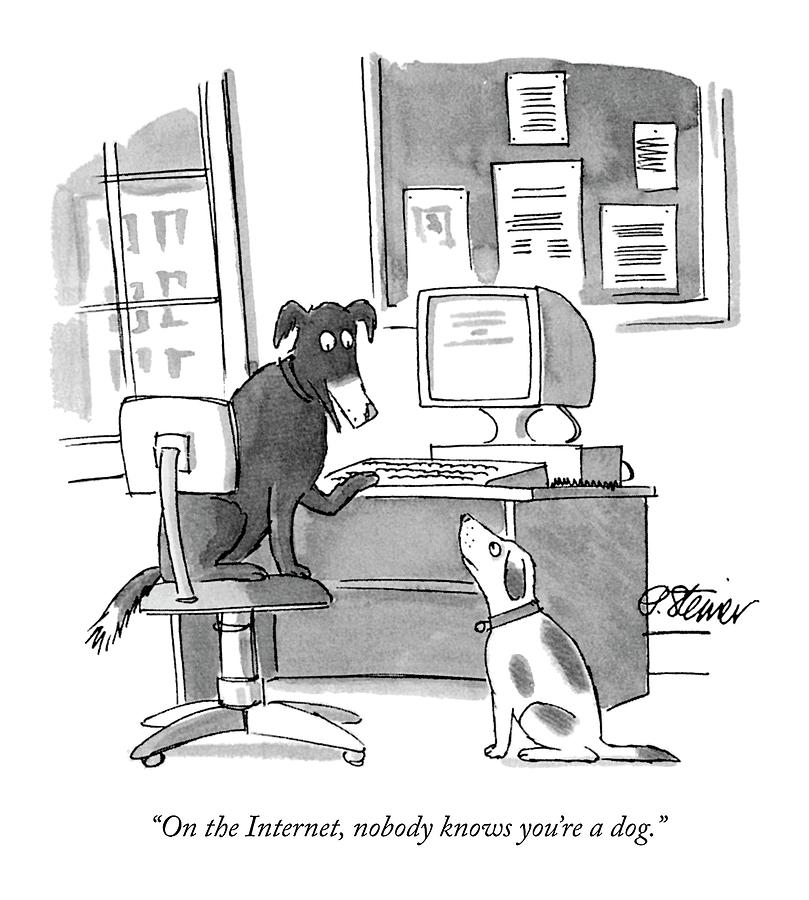
\includegraphics[width=0.6\linewidth]{images/on-the-internet-peter-steine}
	\caption{"On the Internet, nobody knows you are a dog"(\cite{Steiner:Dog:1992})}
	\label{fig:on-the-internet-peter-steine}
\end{figure}

The cartoon of (\cite{Steiner:Dog:1992}) in figure~\ref{fig:on-the-internet-peter-steine}, showing two dogs sitting in front of a computer with the iconic title cited above became an illustration of how people view anonymity on the Internet. Being anonymous on the Internet, however, is not that easy anymore. The use of mobile devices has changed the way how we access information, interact with each other and share content. Digital services are used to access information, which is opening fraught opportunities to attackers who are trying to impersonate someone and access confidential information.  With this change of user behavior, the way we think of authentication and authorization methods has to adjust. Identity management is mandatory to provide a seamless user experience, including identity proofing, authentication, and assertions in federated environments [cf. (\cite{NIST:2017:DIG}), (\cite{Corre:2017:WHI})].


Users find themselves struggling using multiple devices, accounts, and services. The user's burden of this site-by-site account management is putting security at risk. The goal of new authentication and authorization solutions is to help the user managing his accounts by providing single sign-on (SSO), based on an exchange of identity-related assertion across security domains in a scalable way [cf. (\cite{Corre:2017:WHI})].  

In this chapter, existing work and methods to authenticate and authorize users are described. The part is split up in the chapters Security Considerations, Identity Proofing, Authentication, Assertion, Token-based Authentication and SSO Federation Systems.


\section{Security Considerations}
\label{securityConsiderations}

Before getting further into the topic of authentication and authorization, this section will shed light on some basic security principles, concerning authentication and authorization, which help to understand the need for authentication and authorization mechanisms. 

Some basic design principles formulated by Saltzer \& Schroeder (1975) were paraphrased by Neumann (2013) and are still relevant today. The principles give an underlying overview of what should be the focus when designing a secure system. The first of the ten basic security principles formulated by  Saltzer \& Schroeder (1975) is the economy of mechanism which means to keep the design as simple as possible. The next principle describes that access should not be explicitly denied; instead it should be explicitly permitted. For example, when using Access Control Lists (ACLs), all access should be explicitly denied by default. This kind of access control is called Fail-safe defaults.
Furthermore,  Saltzer \& Schroeder (1975) states the complete mediation principle, which states that every access to every object has to be checked for authority without exceptions. A fundamental concept that is part of the basic security principles is open design. The design of an application should not be secret. It can not be assumed that design secrecy will enhance security. This principle is often applied in cryptography. For example, the design of cryptographic algorithms is available for the public, and just the keys remain secret. A broadly used principle in authentication is the separation of privileges. Separation of privileges means that two keys should be used to protect resources if feasible and privileges should be separated.
Every application and user should be provided with least privileges they need to complete their job. The existence of overly powerful mechanisms such as superuser is inherently dangerous - this is called least privilege. The least common mechanism principles compel to minimize the number of mechanisms that common to more than one user are used by all users. In authentication users often get frustrated with the complicated sign-in processes. Therefore, the psychological acceptability should be kept in mind. Keep it simple. The design of the interface for the user should be easy to understand so that the user routinely and automatically applies the protection mechanism correctly. The attack factor or work factor is essential to protect sensitive resources. Cost-to-protect should commensurate with threats and expected risks. It should not be possible to circumvent the mechanism with the resources of the attacker.   
The last one is a recording of compromises which means to provide trails of evidence which are tamper-proof and difficult to bypass. All of these principles are important when choosing an authentication system and need to be considered carefully [cf. (\cite{Neumann:2018:PTC}), (\cite{Saltzer:PICS})]. 

Besides formulating these fundamental principles which will be discussed in various forms,  Saltzer \& Schroeder (1975) also discuss the terms "privacy" and "security". Those terms get frequently used by authors writing about information storing systems, like in this paper. However, the terms "privacy" and "security" are often used very differently.  Saltzer \& Schroeder (1975) for example, defines "privacy" as the ability of an individual to specify whether, when and to whom sensible information is released, and "security" is described as a technique that can control who can modify resources on a computer. Another more recent description of the terms "security" and "privacy" is defined by Brooks et al. (2017). Brooks et al. (2017), states the importance of the distinction between privacy and security. This distinction between privacy and security are essential because there are security issues unrelated to privacy, just as there are privacy issues that are unrelated to security. While security concerns arise from illegal system behavior, privacy concerns arise from byproducts of authorized personally identifiable information (PII) processing. Even byproducts that are considered to protect PII can raise security concerns, for example, it can be questioned to which degree a tool for persistent activity monitoring should reveal information about individuals that are related to security purposes. However, security and privacy have in common that they want to protect personal information and resources or PII [cf. (\cite{Brooks:2017:IPE}), (\cite{Saltzer:PICS})].

These security issues and privacy issues, of course, raise particular concerns for users as well as for companies offering authentication services. When it comes to protecting personal resources, there are three primary concerns. According to Todorov (2007), those three concerns are confidentiality, integrity, and availability. The term confidentiality means that personal information is protected from disclosure to unauthorized individuals and organizations. Integrity or integrity of information, is protecting information from accidental or intentional tampering. Modification of confidential data may affect the data validity. Availability is the need to be able to access information at the time a user requests it. The availability of the services that exposes information has to be given. In an ideal world companies offering authentication and authorization services will do everything to use the best technologies regarding countermeasures to protect confidentiality, integrity, and availability. Establishing countermeasures, however, can be costly leading to a trade-off between costs and level of production of information. A typical approach to establishing information security management is to analyze risks first and then from counter measurements [cf. (\cite{Todorov:2007:MUI})]. 

The paper 'Digital Identity Guidelines' by Grassi, Garcia \& L. (2017), splits the risk assessment into different sections, rather than combining identity proofing, authentication, and federation of digital services into a single Level of Assurance (LOA). In order to provide the most effective approach each of the section is analyzed regarding risk and impacts of failure. The assessment should help to choose security controls and mitigation strategies that help to avoid errors. Errors that can be avoided with an extensive risk assessment among others are identity proofing, authentication and federation errors. Identity proofing risks include a malicious applicant successfully poses as someone else or for example the impacts of collecting more information about an applicant then required. Choosing the right level of assurance in the identity proofing process gives robustness and confidence to the determination of identity. The right authentication assurance level is chosen to mitigate problems in the authentication process, and the binding between an authenticator and a specific individual. An example of a potential error, is the illegal use of someone else's credentials by an applicant. Last but not least, the accurate federation assessment helps to mitigate potential federation errors. Federation errors might occur when an identity assertion is compromised. Analyzing these risks makes it easier to choose an assurance level for each category. Accordingly, the risk gets categorized of harm according to the paper Digital Identity Guidelines by Grassi, Garcia \& L. (2017): 

\begin{itemize}
	\item Inconvenience, distress, or damage to standing or reputation
	\item Financial loss or agency liability
	\item Harm to agency programs or public interests
	\item Personal safety
	\item Civil or criminal violations
\end{itemize}

Each of the categories can then be rated with a potential impact level which can be either low, moderate or high. The result of this risk assessment can then be the basis for choosing the appropriate identity, authentication and federation assurance level. The assurance level determination is just relevant for analyzing the risk of online transaction offered by digital services and should not be used for the complete business process which may include offline processing in an entirely segmented system [cf. (\cite{NIST:2017:DIG})]. 

The result of all design principles, security and privacy considerations should be a system, network or component that is trustworthy. According to Neumann (2018), trustworthiness is given if an entity satisfies its specified requirement, after a reliable assessment. The requirements that deserve special consideration are, those that are critical to an enterprise, mission, system, network or other entity. One of the requirements to make a system trustworthy is a reliable authentication and authorization process. These processes are discussed in more detail in the next sections [cf. (\cite{Neumann:2018:PTC})].



\section{Identity Proofing}
\label{identityProofing}

“Digital identity is the unique representation of a subject engaged in an online transaction. The process used to verify a subject’s association with their real-world identity is called identity proofing” (\cite{NIST:2017:DIG})

A digital identity as explained above is the result of what is called the authentication process. It is a way of identifying the user as who they claim to be. In order to prove the user's identity presentation, validation and verification of a minimum set of attributes are necessary [cf. (\cite{Boyd:2012:GSOAuth})]. 

To become authenticated, the user has to go through certain steps on the way. These steps are enabled by typical components unique to the authentication process. Todorov (2007) identifies three typical components that are part of the authentication of the Supplicant, the Authenticator, and the Security Database. The Supplicant is the party that provides the evidence to prove the identity of a user or client. The result of the authentication process should be the authenticated user or client. The Authenticator, is responsible for ascertaining the user identity. After proving the identity, the authenticator can authorize or audit the user access to resources. The Security Authority Database is a storage or a mechanism to check the user's credentials. The storage can be represented by as much as a flat file, a server on the network providing centralized user authentication or a distributed authentication server [cf. (\cite{Todorov:2007:MUI})]. 



\begin{figure}[h]
	\centering
	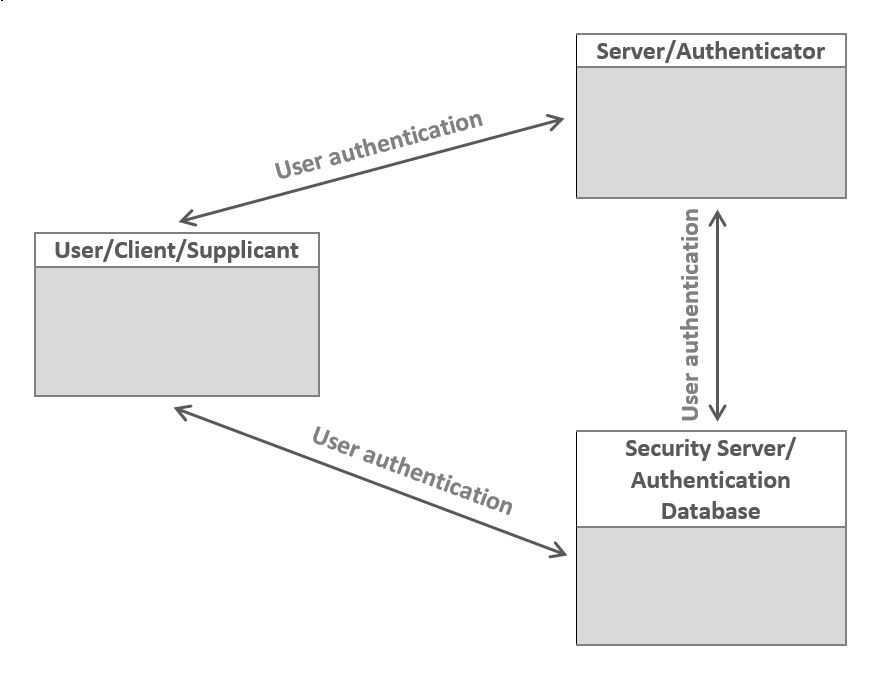
\includegraphics[width=0.8\linewidth]{images/identity_proofing_architectur}
	\caption[Componets Authentication]{Components of User Authentication System (\cite{Todorov:2007:MUI})}
	\label{fig:componentsuserauthenticationsystem}
\end{figure}

It is vital that all the components as shown in figure~\ref{fig:componentsuserauthenticationsystem}, of a user authentication system can communicate independently of each other. Whether or not all communication channels are used, depends on the authentication mechanism and the model of trust that it implements. For example, the Kerberos authentication protocol does not feature direct communication between the authenticator and security server [cf. (\cite{Todorov:2007:MUI})]. 

The paper 'Digital Identity Guidelines - Enrollment and Identity Proofing' by Grassi, J.L. Fenton, et al. (2017) also describes components that are similar to the ones described by Todorov (2007) in figure~\ref{fig:componentsuserauthenticationsystem}. Furthermore the paper 'Digital Identity Guidelines - Enrollment and Identity Proofing' by Grassi, J.L. Fenton, et al. (2017) describes three different identity assurance level shown in table~\ref{tab:ial}. These assurance level state to which degree identity assurance can or should be provided in a system [cf. (\cite{NIST:2017:DIGEIP}), (\cite{Todorov:2007:MUI})]. 


\begin{table}[h]
	\centering
	\begingroup
	\setlength{\tabcolsep}{10pt} % Default value: 6pt
	\renewcommand{\arraystretch}{1.5} % 
	\begin{tabular}{cl}
		\hline
		\multicolumn{2}{c}{\cellcolor[HTML]{656565}{\color[HTML]{FFFFFF} Identity Assurance Level}}                                                                                                                                                                   \\ \hline
		\multicolumn{1}{|c|}{\textbf{IAL1}} & \multicolumn{1}{l|}{\begin{tabular}[c]{@{}l@{}}There is no need to link the applicant to a real-life identity.   All\\ attributes provided are self asserted and are neither validated nor \\ verified.\end{tabular}}   \\ \hline
		\multicolumn{1}{|c|}{\textbf{IAL2}} & \multicolumn{1}{l|}{\begin{tabular}[c]{@{}l@{}}The evidence provided supports the real-world existence of the \\ claimed identity. The identity proofing has to be either  remote \\ or physical present.\end{tabular}} \\ \hline
		\multicolumn{1}{|c|}{\textbf{IAL3}} & \multicolumn{1}{l|}{\begin{tabular}[c]{@{}l@{}}The identity proofing requires physical presence. Attributes must\\ be verified by a authorized and trained CSP.\end{tabular}}                                            \\ \hline
	\end{tabular}
	\endgroup
	\caption{Identity Assurance Levels (\cite{NIST:2017:DIG}, p.18)} \label{tab:ial}
\end{table}
\pagebreak[4]
Moreover, the paper 'Digital Identity Guidelines - Enrollment and Identity Proofing' by Grassi, J. L. Fenton, et al. (2017), describes additional expectations of the identity proofing process. The expected outcome of the identity proofing process should be that the claimed identity is linked to a single, unique identity. The provided evidence for the claimed identity has to be validated. The validation should prove that the evidence is correct, genuine and exists in the real world.
This section describes certain aspects of the authentication process and gives a very general description of components that can be part of an authentication process. Furthermore, identity proofing assurance level is provided that are relevant for the risk assessment. This chapter describes that the user has to provide proof of the claimed identity but lacks to describes how this provided proof might look and how it is validated – this is described in the next section~\ref{authentication} [cf. (\cite{NIST:2017:DIGEIP})].
	

\section{Authentication}
\label{authentication}
For a very typical authentication process, the user provides its username and password when the application demands it. If the user provides a correct username and password, an application assumes that the user is indeed the owner of the account. The evidence provided by the user in the authentication process is called credentials. Most of the time, as mentioned above, credentials get provided in the form of username and password. Nevertheless, credentials may as well take other forms like Personal Identification Numbers (PIN), key cards, eye scanners and so on [cf. (\cite{Todorov:2007:MUI}), (\cite{Boyd:2012:GSOAuth})]. 

Credentials, which prove the identity of an entity and find use as authenticators in authentication systems, are called factors. The 'Digital Identity Guidelines' by Grassi, Garcia \& L. (2017) categorizes the following types of factors:

\begin{itemize}  
	\item Something, the user, knows - Cognitive information the user has to remember. Examples include passwords, PIN, answers to secret questions.
	\item What the user has - something the user owns. Examples include a security token, driving license, one-time password (OTP). 
	\item What the user is - biometric information of the user. Examples include fingerprint, voice, and face. 
\end{itemize}

Other types of information which are not considered authentication factors but  can be used to enrich the authentication process according to Dasgupta, Arunava \& Abhijit (2017) are:

\begin{itemize}
	\item Where the user is - the location of the user can is used as a fourth factor of authentication. Examples include GPS, IP addresses.
	\item When the user logs on - Time can also be extracted as a separate factor. Verification of employee’s identification in different office hours can prevent many kinds of grave data breaches. The time factor can easily prevent online banking fraud events to a great extent. 
\end{itemize}

The authenticators are based on secrets that can be either public key pairs (asymmetric keys) or shared secrets (symmetric keys). Public key pairs consist of a private and a public key. The private key gets stored on the authenticator. The holder of the private key can use it to prove they control the authenticator. The verifier of the authenticator can then use the public key - most likely received with the help of a public key certificate - together with the authentication protocol to verify the identity of the user. Shared secrets can be either symmetric keys or memorized secrets. Both keys and passwords can be used with similar protocols. However, there is a huge difference for the user. Symmetric keys are generally stored on hardware; secrets have to be memorized by the subscriber which can lead to multiple vulnerabilities. Cryptographic keys are typically long enough to make network-based guessing attacks untenable but if the user chooses short, memorable passwords the system may be vulnerable [cf. (\cite{NIST:2017:DIG}), (\cite{Dasgupta:2017:AUA})]. 


To secure a solution properly, it should at least use two factors of the three listed above. To make use of more than one factor of a pool of potential credentials to verify the identity of a user is referred to as Multi-factor Authentication (MFA). The goal of multi-factor authentication is to provide a layered defense and make it harder for unauthorized individuals to gain access. If one of the factors breaks, the service can still rely on the non-compromised authentication factors [cf. (\cite{Dasgupta:2017:AUA})].

Using just one factor is called Single Factor Authentication(SFA). Dasgupta, Arunava \& Abhijit (2017) clearly describes the drawbacks SFA has compared to MFA, primarily the universal used password-based authentication. The user needs to remember different passwords for multiple accounts. Therefore, the user often reuses one password also known as password fatigue [cf. (\cite{Dasgupta:2017:AUA})].

In an Interview by Tomkins (2009) with Jon Brody, he explains Password Fatigue like the following. An average user has 15 accounts; some people might even have up to 30 accounts - far too much to manage appropriately. Users then tend to adopt specific password patterns like using simple passwords for nontransactional sites and complex passwords for banking sites. Since many complex passwords are hard to remember users also often reuse passwords for different services at one point - this is called password fatigue [cf. (\cite{Tomkins:2009:DPF})]. 

Besides password fatigue Todorov (2007) draws attention to one of the significant challenges of secure user authentication represented by default passwords. Vendors often ship their devices with pre-configured standard passwords. Although vendors recommend changing default passwords, system architects and engineers often fail to do so because they are more focused on the business logic than on security causing security issues. Systems with default passwords are more straightforward to attack, for example by knowing or guessing the device the attacker has an easy time authenticating with the system accordingly [cf. (\cite{Todorov:2007:MUI})]. 


Due to the problem of password fatigue and default passwords, one factor like a password might easily gets compromised. The user can then no longer use the service until the repair of the system which can lead to a delay of the user when trying to access necessary information. Also, there is a risk that the user does not notice the compromise of the single factor which can lead to devastating effects [cf. (\cite{Dasgupta:2017:AUA})]. 


\begin{table}[h]
	\centering
	\begingroup
	\setlength{\tabcolsep}{10pt} % Default value: 6pt
	\renewcommand{\arraystretch}{1.5} % 
	\begin{tabular}{cl}
		\hline
		\multicolumn{2}{c}{\cellcolor[HTML]{656565}{\color[HTML]{FFFFFF} Authenticator Assurance Level}}                                                                                                                                                                                                                                                                                                                                     \\ \hline
		\multicolumn{1}{|c|}{\textbf{AAL1}} & \multicolumn{1}{l|}{\begin{tabular}[c]{@{}l@{}}The first level defines that a claimant has to provide some kind of\\ assurance that they control an authenticator bound to a subscriber's\\ account through a secure authentication protocol. The guarantee can be\\ either in the form of a single-factor or multi-factor authentication.\end{tabular}}                                         \\ \hline
		\multicolumn{1}{|c|}{\textbf{AAL2}} & \multicolumn{1}{l|}{\begin{tabular}[c]{@{}l@{}}The second level requires the use of at least two distinct authentication\\ factors. The confidence that the claimant controls the authenticators of\\ the subscriber's account is high at this level. Appropriate cryptographic\\ techniques are required.\end{tabular}}                                                                     \\ \hline
		\multicolumn{1}{|c|}{\textbf{AAL3}} & \multicolumn{1}{l|}{\begin{tabular}[c]{@{}l@{}}The third level provides a very high level of confidence that the claimant\\ is in possession of the authenticators bound to the subscriber. Claimants\\ need to prove possession of the key with two distinct authenticators\\ through a secure authentication protocol. One of the authenticators needs\\ to be hardware-based.\end{tabular}} \\ \hline
	\end{tabular}
	\endgroup
	\caption{Authenticator Assurance Levels (\cite{NIST:2017:DIG}, p.19)} \label{tab:aal}
\end{table}
\pagebreak[4]
When designing an authentication process by using multiple factors the designers of the process should be acutely aware of the type of application and the information that has to be secured. For example, a solution for an international bank should have different standards than an application for a maintaining a grocery list. On the one hand, challenging and complex authentication processes for trivial applications might scare away users. On the other hand, simple methods for applications protecting sensitive data might drive users away as well. Application designers should always try to find a middle way that suits both parties, the application owners and the users [cf. (\cite{NIST:2017:DIG})]. 


Furthermore the paper 'Digital Identity Guidelines - Authentication and Lifecycle Management' by Grassi, J. Fenton, et al. (2017) defines three different authenticator assurance levels to make sure the system a company is designing uses the appropriate authenticators for their purpose. Each of the authenticator assurance levels has to fulfill all the requirements of their successor. The paper 'Digital Identity Guidelines - Authentication and Lifecycle Management' by  Grassi, J. Fenton, et al. (2017) describes three levels shown in table~\ref{tab:aal} [cf. (\cite{NIST:2017:DIGAL})].

Authentication is a critical part of every application. As users are getting more concerned on security, the pressure on developers grows to provide a solution that secures sensitive data while keeping up usability standards, which can often be a trade-off. Complex applications need complex security which can mean high costs for individually developed solutions; therefore application developers should also think about using federated authentication solutions [cf. (\cite{NIST:2017:DIGAL})].


\section{Assertion}
\label{assertion}
The authentication and authorization process are very closely related to each other and for users often hard to separate. After the authentication process of a user, the application has now proved that the user is who they claim to be, but not every user is the same. After the user authenticates, the user may want to access data or services. Based on the information provided by the authentication process the application can allow or deny the user to access information or services. In other words, it needs to be evaluated if the user is authorized to access data from a service. Furthermore, authorization offers granular control to distinguish between read, write or execute access to individual resources, typically access control lists (ACL) are used for each operation [cf. (\cite{Todorov:2007:MUI}), (\cite{Boyed:2012:GSOA})].

Systems offer a user login process or sign-in process, in order to receive the information necessary to make authorization decisions. The login process initiates the authentication process between the user and the system. As a result of this process where the user has to prove their identity, the user receives a system or application specific structure. In a federated identity system, this is called an assertion. The assertion holds an identifier and identification information about the user which can indicate for example what kind of resources the user can access. For every action, the user then has to provide the assertion and based on the information provided within the assertion the user is then either granted or denied access. Another example of the usage of the assertion is the personalization of websites [cf. (\cite{Todorov:2007:MUI}), (\cite{NIST:2017:DIG})].

In federated systems, the verifier of authentication information of the user is called Identity Provider (IdP), and the party that receives and uses information is called the Relying Party(RP). In the context of the federated identification systems the user, or the one that is trying to access information from a system is called the subscriber. The IdP generates an assertion for the verifier associated with the subscriber. This process allows subscribers to access multiple RPs without maintaining separate credentials and the process also supports SSO [cf. \cite{NIST:2017:DIGFA}].

The paper 'Digital Identity Guidelines - Federation and Assertion' by Grassi, Richer, et al. (2017), defines different levels of federation assurance that define how assertion should be constructed and secured for a given transaction. Each successive level has to fulfill the requirements of all lower level. Federation assurance levels defined by the paper 'Digital Identity Guidelines - Federation and Assertion' by Grassi, Richer, et al.  (2017) are shown in table~\ref{tab:fal}.



\begin{table}[h]
	\centering
	\begingroup
	\setlength{\tabcolsep}{10pt} % Default value: 6pt
	\renewcommand{\arraystretch}{1.5} % 
	\begin{tabular}{cl}
		\hline
		\multicolumn{2}{c}{\cellcolor[HTML]{656565}{\color[HTML]{FFFFFF} Federation Assurance Level}}                                                                                                                                                                                                                                                                   \\ \hline
		\multicolumn{1}{|c|}{\textbf{FAL1}} & \multicolumn{1}{l|}{\begin{tabular}[c]{@{}l@{}}The first level requires a bearer assertion, signed with approved cryptography\\ by an IdP, for example, OpenID Connect Basic Client profile or Security As-\\ sertion Markup Language (SAML) Web SSO Artifact Binding profile with no\\ additional feature.\end{tabular}} \\ \hline
		\multicolumn{1}{|c|}{\textbf{FAL2}} & \multicolumn{1}{l|}{\begin{tabular}[c]{@{}l@{}}The second level requires an assertion like the OpenID Connect ID Token or\\ SAML Assertion, to be encrypted with the public key of the RP, whereas the\\ RP is the only party that can decrypt the bearer assertion.\end{tabular}}                                        \\ \hline
		\multicolumn{1}{|c|}{\textbf{FAL3}} & \multicolumn{1}{l|}{\begin{tabular}[c]{@{}l@{}}Additonally to the first two levels the last federation assertion level requires\\ the subscriber to prove their possession of a key that is bound to the\\ assertion (holder of key assertion) and initially was used to authenticate to\\ the IdP.\end{tabular}} \\ \hline
		
	\end{tabular}
	\endgroup
	\caption{Federated Assurance Levels (\cite{NIST:2017:DIG}, p.19)} \label{tab:fal}
\end{table}

For any assertion level, the IdP has to make sure that an RP cannot impersonate the IdP at another RP by signing the assertion. The signing of the assertion can be done by either a Media Access Control (MAC) using a shared key or a digital signature using an asymmetric key [cf. (\cite{NIST:2017:DIG}), (\cite{NIST:2017:DIGFA})].  

One of the factors that differentiate the federation assurance level is the usage of assertion binding. An assertion binding can be chosen based on the RP requirements. It may be required for example that the RP needs additional proof of the binding of an assertion to a particular subscriber. The two different kinds of assertion binding to chose from is the bearer and holder-of-key assertions. Any party can present a bearer assertion in order to prove they have the identity of the bearer. Based on this handling of bearer assertions it can be assumed, that if an attacker is successful in capturing a bearer assertion, the attacker can represent the subscriber that was previously associated with this bearer assertion. The attacker could present the assertion or reference to the RP and impersonate the subscriber. The holder-of-key assertion in comparison holds a reference to a key which indicates which subscriber is representing the assertion. The key is signed and asserted by the issuer of the assertion [cf. (\cite{NIST:2017:DIGFA})].

Typically tokens are used for assertions, in this context, tokens are software tokens which are used to provide access control for systems. The assertion binding described before can also be referred to as token profiles. Typically there are two kind of tokens that are frequently used, which is the access token and the refresh token. An access token, when it is valid can be used to access resources. If the access token is expired and not valid anymore a refresh token can be used to reclaim a new access token. OpenID Connect additionally defines an ID token which will be discussed later [cf. (\cite{Spencer:2018:APISecurity})]. 

Furthermore, tokens can be passed either by reference or by value. On the one hand, if tokens are passed by reference, they have to be resolved in another instance. On the other hand, a token can be passed by value and already has all the necessary information about the user to establish for example a session. Those two ways of passing a token are significant when it comes to security considerations. Also, tokens have different types. The OAuth specification, for example, does not specify which kind of token has to be used. Spencer (2018), lists some of the typical tokens: 

\begin{itemize}
	\item WS-Security token (SAML)
	\item JSON Web Tokens (JWT)
	\item Legacy tokens
	\item Custom tokens
\end{itemize}

In praxis developers often use JWT's because they are very flexible and allow to add additional claims. Also, they use JavaScript Object Notation (JSON) and not Extensible Markup Language (XML) like SAML tokens, which is much easier to process. More about JSON Tokens can be read in the upcoming chapter Token-based Authentication [cf. (\cite{Spencer:2018:APISecurity})].

\section{Token-based Authentication}
\label{tokenBasedAuthentication}

The way web developers write back-end applications has changed significantly with the rising popularity of single page and mobile applications. Backend-developers no longer spend a lot of time building a markup. Instead, they build APIs for frontend applications to consume. The split up of frontend and backend allows the backend to focus on business logic and data management while the frontend solely focus on the representation of the content. The number one way single page and mobile web applications are authenticating users according to Tkalec (2015) is token-based authentication [cf. (\cite{Tkalec:2015})].  

Serilleja (2015) shares the view that token-based authentication is the modern way to handle authentication. Token-based authentication should be considered because of various factors. It is optimal for mobile applications which work in a stateless way and need to adapt to the sudden change of demand in a scalable way. Furthermore, token-based authentication provides extra security and applications can pass on authenticated users to other applications. Serilleja (2015) and Tkalec (2015) concluded that token-based authentication is the best alternative for modern web applications to authenticate their users. Serilleja (2015) examines how authentication was done in the past to show difficulties and limits past approaches had and highlight the advantages of token-based authentication. One approach to authenticate users, used in the past is server-based authentication [cf. (\cite{Serilleja:2015:Scothio}), (\cite{Tkalec:2015})]. 

\subsection{Server-Based Authentication.}
A lot of modern-day API’s built on the Representational State Transfer (REST) programming paradigm which basis is the Hypertext Transfer Protocol (HTTP) which is stateless as well. A protocol that is stateless does not recall the actions that were taken beforehand which mean for example that if we authenticate the user, in the next request we have to authenticate the user again because the application will not know the user anymore [cf. (\cite{Serilleja:2015:Scothio})]. 

The aim of server-based authentication is for the application to remember the user that logged on at the application. The application has to store the information on the server, which can be done in a few different ways during the session, usually in memory on the disk. The workflow of a server-based authentication starts with the server delivering the website and the user logging in with username and password. The server saves the information from the user login info in a session. After the session is established, the session is checked on the server for every request. If the session is valid, the server returns the requested data to the client. However, since modern Single Page Applications (SPA) and mobile applications are on the rise, this method to authenticate users shown some problems, especially when it comes to scalability [cf. (\cite{Serilleja:2015:Scothio})]. 

The session handling with server-based authentication is especially hard on the server’s bandwidth. Most of the time the session gets established in memory on the server when the user authenticates. This approach leads to an enormous overhead. The second problem with this approach is that the information of the user is also held in memory on the server. Since more and more companies are moving servers to the cloud, this is not only a security issue, also replicating servers for scale is limited. Also nowadays users want to access their data at any moment from every device. Providing the user with the possibility to access data across multiple mobile devices is vital, which means cross-origin resource sharing has to be enabled. With server-based authentication, it is possible to run into problems with cross-origin request [cf. (\cite{Serilleja:2015:Scothio})].


\subsection{
	Token-based authentication with JSON Web Token
}

The most important thing about token-based authentication is that it is stateless, much like HTTP. The server does not have to hold the session of the user over an extended period on the server. Instead, the user can request resources by offering a token generated by an authentication server. The token sent in the query string or authorization header, can then be validated at the resource server and the secure resource will be returned to the user. The approach of using JSON Web Tokens (JWT) provides the ability to scale applications without considering on which domain the user logged in. Another advantage besides being scalable is that token-based authentication gives one the possibility to reuse the same token for authenticating the user. Therefore, it gets easier to build applications that share permission with other application because many separate servers, running on multiple platforms and domains can reuse the same token. The approach also gives performance advantages compared to server-side authentication because there is no need to find and deserialize the session on each request. However, since it is best practice to encrypt the token, the token still needs to be validated, and the content needs to be parsed. One way to implement token-based authentication is with the help of JWT's. JWT's are gaining popularity fast and are backed by huge companies like Google and Microsoft. Also, the Internet Engineering Task Force defines a standard specification for JSON Web Tokens. OpenID and OAuth also use JWT as a standard; therefore, the usage of the JWT will be explained in detail [cf. (\cite{Tkalec:2015})].



JWT is a compact structure that holds information about the authentication of a user or claims. The structure is indented for space-constrained environments such as HTTP Authorization headers. The payload of JWT is of JSON, enabling the claims to be digitally signed or integrity protected with a MAC and encrypted [cf. (\cite{JWT:IETF:Jones:2015})].

The standard is used to transport data between interested parties. The transferred data can be for example the identity of a user or user’s entitlements. Furthermore, with the possibility of digital signatures and encryption, data can be transferred securely over an unsecured channel. The signatures also allow asserting the identity of a user if the recipient trusts JWT is asserting party [cf. (\cite{Siriwardena:JWTJWSJWE:2016})].

An example of a JWT is an id\_token. Google provides an OAuth 2.0 Playground for Developers, where scopes can be chosen and tried out against the Google API. To get an excellent example of a JWT, OAuth2 API v2 was selected and authorized like shown in figure~\ref{fig:googleoauthplaygroundoauthapi} [cf. (\cite{Google:2018:OAuthPlayground})].


\begin{figure}[h]
	\centering
	
\includegraphics[width=0.8\linewidth]{images/googleOAuthPlaygroundOAuthAPI}
	\caption[OAuth API]{Google Developers Playground OAuth 2.0 API}
	\label{fig:googleoauthplaygroundoauthapi}
\end{figure}

After choosing and authorizing with a Google Account, the Google API returns an Authorization Code. This Authorization Code is specific for a certain Authentication Flow defined by OAuth and can then be exchanged for the tokens. As a result, all information for the scopes that were selected beforehand is returned. Because OAuth 2 API v2 was selected, the returned value is an id\_token. This id\_token is a nice representation of a JWT and holds the standard information that is required according to the OAuth specification  [cf. (\cite{Google:2018:OAuthPlayground})].

\lstset{caption=JWT Token,breaklines=true, breakatwhitespace=true, basicstyle=\small\ttfamily, label={lst:jwt}, tabsize=3, basewidth={0.55em}, fontadjust, language=XML}
\begin{lstlisting}
eyJhbGciOiJSUzI1NiIsImtpZCI6ImRhZDQ0NzM5NTc2NDg1ZWMzMGQyMjg4NDJlNzNh
Y2UwYmMzNjdiYzQifQ
.
eyJhenAiOiI0MDc0MDg3MTgxOTIuYXBwcy5nb29nbGV1c2VyY29udGVudC5jb20iLCJh
dWQiOiI0MDc0MDg3MTgxOTIuYXBwcy5nb29nbGV1c2VyY29udGVudC5jb20iLCJzdWIi
OiIxMTIzMDE5MzgzMjI4MTAyMzk3MTIiLCJlbWFpbCI6ImNvcm5lbGlhcmF1Y2hAZ214
LmF0IiwiZW1haWxfdmVyaWZpZWQiOnRydWUsImF0X2hhc2giOiJSdjJRQjZoZzFqdDZR
aHRJWG5laWVnIiwiZXhwIjoxNTI5NzQ3MTk2LCJpc3MiOiJodHRwczovL2FjY291bnRz
Lmdvb2dsZS5jb20iLCJpYXQiOjE1Mjk3NDM1OTYsIm5hbWUiOiJDb25ueSBSYXVjaCIs
InBpY3R1cmUiOiJodHRwczovL2xoNC5nb29nbGV1c2VyY29udGVudC5jb20vLWJFbEt3
aDVaNUJnL0FBQUFBQUFBQUFJL0FBQUFBQUFBQk5rL0p5Qm1XTW9uYUlJL3M5Ni1jL3Bo
b3RvLmpwZyIsImdpdmVuX25hbWUiOiJDb25ueSIsImZhbWlseV9uYW1lIjoiUmF1Y2gi
LCJsb2NhbGUiOiJkZSJ9
.
yibOtrXy9_-cfOWytzwGuE4zqLv-MK_2-PYIKR_xecJt9ACnMnNMSmio6i8Vu7U061wF
OTb-qRennHbvy3lTRZLcTXttIrIUl-NdnZs2BrTSGWrw9aRzEjIHAXiY4fGRHj9VZXs_
_J3Nn0EoBmT7Cnua2hb4U_X3hAyGpEvlSGKc5HvbyzOAtNh081Cyj1TI-AidCPTuC5vh
68C55tLJ87PWNm8WU1rCPOPBdVTjhYlqJKCpgUJ39_p_MXL_uHBZXRrvbOyV_tZVlw47
rjd8GFnBq1QqsYAR-6wrFbNL1pY6tPyriqZnQdi5KqYWPUwGpXbFDUfhZAmWXT8-PTsc
gQETEp8o3RvRHtfSu8Gx4UOhukt9_VxVdHmpFw
\end{lstlisting}

\goodbreak

The JWT Token in the listing~\ref{lst:jwt} is presented as a sequence of URL-save base64url-encoded values. The different values are separated by a (‘.’) character. How many parts a JWT has is dependent on how the JWT is serialized. Either by using the JWS Compact Serialization or JWE Compact Serialization [cf. (\cite{JWT:IETF:Jones:2015})].


To understand this JWT token in the listing~\ref{lst:jwt} it is best to look at each of the three parts of the JWT separately. When decoding the first part of the JWT, we receive a JSON object. Each part can be decoded individually but if a quick representation of a token is needed developers are the best advised to use \href{https://jwt.io/} {https://jwt.io/}. The website not only decodes the information of the token it also verifies the token. The website shows a warning if the token is not flawless according to the JWT specification. The verification of the token and the signing is done with multiple libraries that provide information about certain vulnerabilities of the JSON Web Token. The first decoded part of the JWT gives us the following JSON [cf. (\cite{JWT:IETF:Jones:2015})].


\lstset{
	caption=JOSE Header,
	label={lst:joseheader},
	string=[s]{"}{"},
	stringstyle=\color{blue},
	comment=[l]{:},
	commentstyle=\color{black}
}
\begin{lstlisting}
{
"alg": "HS256",
"typ": "JWT"
}
\end{lstlisting}


The JSON object in listing~\ref{lst:joseheader} is the JOSE Header, representing the type of the token, the cryptographic operations applied and optionally additional properties of the JWT. Based on the information of the JOSE Header it can explain if the JWT is a JWS or a JWE. When speaking of JWT, we speak of one of the implementations of JWT because in fact, JWT does not exist itself. Concrete implementation of the JWT is JSON Web Signature (JWS) or JSON Web Encryption (JWE). The figure~\ref{fig:jwtjwsjwe2} gives an optical representation of the structure [cf. (\cite{Siriwardena:JWTJWSJWE:2016})].


The 'type' Header Parameter we can examine in listing~\ref{lst:joseheader} indicates the kind of token, considering the example it is a JSON Web Token. The second parameter is the 'alg' Header Parameter and is specified in either the 'JSON Web Security (JWS)' reference documentation written by Jones, Bradley \& N. (2015) or the 'JSON Web Encryption (JWE)' reference documentation written by Jones \& Hilbrand (2015). In this case, the JWT is a JWS since a JWE needs more specific Header Parameter. In the JWS the 'alg' Header Parameter gives information about the algorithm which was used to create the signature. Which kind of arguments are accepted by the 'alg' Header Parameter are explained in yet another specification called 'JSON Web Signature and Encryption Algorithms' written by Jones (2015). In the listing~\ref{lst:joseheader} the 'HS256' algorithm is used, meaning that the JWS was MACed using the HMAC SHA-256 algorithm. The definition of the 'alg' Header Parameter in the 'JSON Web Signature (JWS)' reference documentation is very similar to the definition in the 'JSON Web Encryption (JWE)' reference documentation by Jones \& Hilbrand (2015) except the cryptographic algorithm is used to encrypt or determine the value of the Content Encryption Key (CEK). Jones \& Hilbrand (2015), also defines an 'enc' Encryption Algorithm Header, which is used for content encryption on plaintext. The authenticated encryption performed produces a ciphertext and the authentication tag. Also for the 'enc' Header Parameter, the valid arguments can be found in the 'JSON Web Signature and Encryption Algorithms' written by Jones (2015). The algorithm used must be an AEAD algorithm with a specified key length. There is further Header Parameter that can be defined, here are just the essential JOSE Header Parameter for this document listed [cf. (\cite{JWE:IETF:Jones:2015}),( \cite{JWA:Jones:2015}), (\cite{JWS:IETF:Jones:2015})]. 

\begin{figure}[h]
	\centering
	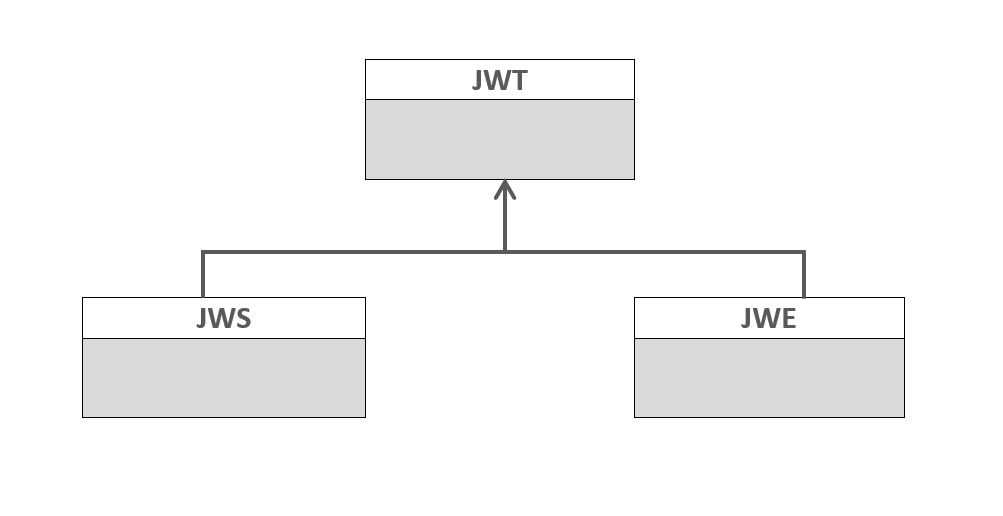
\includegraphics[width=0.8\linewidth]{images/jwtjwsjwe2}
	\caption{JWT Inheritance}
	\label{fig:jwtjwsjwe2}
\end{figure}

The second decoded part of the example in listing ~\ref{lst:jwt}, represents the claim set. The representation of the claim set is a JSON, where each key has to be unique. If the keys are duplicated a JSON parsing can occur or the last one of the duplicated keys is returned. 
\pagebreak[4]

\lstset{
	caption=Claim Set,
	label={lst:claimset},
	string=[s]{"}{"},
	stringstyle=\color{blue},
	comment=[l]{:},
	commentstyle=\color{black}
}
\begin{lstlisting}
{
"azp": "407408718192.apps.googleusercontent.com",
"aud": "407408718192.apps.googleusercontent.com",
"sub": "112301938322810239712",
"email": "corneliarauch@gmx.at",
"email_verified": true,
"at_hash": "Rv2QB6hg1jt6QhtIXneieg",
"exp": 1529747196,
"iss": "https://accounts.google.com",
"iat": 1529743596,
"name": "Conny Rauch",
"picture": "https://lh4.googleusercontent.com/-bElKwh5Z5Bg/
AAAAAAAAAAI/AAAAAAAABNk/JyBmWMonaII/s96-c/photo.jpg",
"given_name": "Conny",
"family_name": "Rauch",
"locale": "de"
}
\end{lstlisting}

The decoded value from the example in listing~\ref{lst:jwt} of the Google OAuth 2.0 Playground  by Google (2018), returns a JSON object shown in the listing \ref{lst:claimset}. The claim set we receive is composed of mandatory and optional claims. Specifically requested in this example were the login, email and profile scope which affected the claims returned from the Google OAuth 2.0 API. Mandatory claims for the login with OpenID are iss, iat, aud, sub and exp and an optional claim that was returned from the API is azp. For the profile scope, the specific claims that were returned are name, picture, given\_name, family\_name, and locale. Email specific claims are email and email\_verified. Furthermore, identity providers can include additional elements that are neither mandatory or optional claims [cf. ({\cite{Google:2018:OAuthPlayground}), (\cite{Siriwardena:JWTJWSJWE:2016})]}].

The last and third part from the example in listing \ref{lst:jwt}  represents the base64url-encoded signature. To know which kind of signature the decoded code is resembling a peek at the JOSE Header will help. The JOSE Header as mentioned before gives information about the cryptographic elements that were used related to the signature. In case of listing~\ref{lst:signaturejwt} the Google OAuth 2.0 API uses RASSSA-PKCS1-V1\_5 with the SHA-256 hashing algorithm. However, the \href{https://jwt.io/} {https://jwt.io/} website does not provide us with the decoded public key. 
\pagebreak[4]

\lstset{
	caption=Signature JWT,
	label={lst:signaturejwt},
	string=[s]{"}{"},
	stringstyle=\color{blue},
	comment=[l]{:},
	commentstyle=\color{black}
}
\begin{lstlisting}
{
RSASHA256(
base64UrlEncode(header) + "." +
base64UrlEncode(payload),
Public Key or Certificate.
)
}
\end{lstlisting}


To serialize an encrypted message, one has to follow either the JWS or the JWE specification. Each of the specifications has the type’s compact serialization. Google OpenID Connect uses the compact serialization. The OpenID Connect specification suggest using the JWS compact serialization or the JWE compact serialization. In this paper only the compact serialization will be discussed, the specification of the other serialization method can be either looked up in the JWE specification or the JWS specification. To call a JWS or a JWE, a JWT has to follow the compact serialization [cf. (\cite{JWS:IETF:Jones:2015}), ({\cite{JWE:IETF:Jones:2015})].
	
	The aim of the JWS Compact Serialization is it to present content as a compact, URL-safe string, which is either digitally signed or MACed. It is not possible to use multiple signature or MAC in a JWS Compact Serialization and furthermore it is not allowed to use JWS Unprotected Headers. An unprotected header is a JSON object which includes the header element that is not integrity protected, which concludes that a protected header is a JSON object that is integrity protected by using MAC or digital signatures. A JWS Compact Serializations is represented as a concatenated string shown in listing~\ref{lst:jwscompactserialization} [cf. (\cite{JWS:IETF:Jones:2015})].
	
	\lstset{
		caption=JWS Compact Serialization,
		label={lst:jwscompactserialization},
		string=[s]{"}{"},
		stringstyle=\color{blue},
		comment=[l]{:},
		commentstyle=\color{black}
	}
	\begin{lstlisting}
	{
	BASE64URL(UTF8(JWS Protected Header)) '.'
	BASE64URL(JWS Payload) '.'
	BASE64URL(JWS Signature)
	}
	\end{lstlisting}
	
	The first element is called the JOSE header which contains all the information that advertises the public key corresponding to the private key that was used to sign the message. Elements of the header include the jku, jwk, kid, x5u, x5c, x5t and x5t\#s256. The second element is the JWS Payload or the content to be signed, which does not have to be JSON. The following approach is used  to construct the message: ASCII(BASE64URL-ENCODE(UTF8(JOSE Header)) '.' BASE64URL-ENCODE(JWS Payload)). 
	The last element is the JWS signature, which is computed over the message that was constructed beforehand, using the algorithm defined in the JOSE Header. These three key components together are called a JWS token. When using the JWE Compact Serialization, the output is called JWE token. Compared to the JWS token, which we saw above the JWS token consists of 5 different key components [cf. (\cite{JWS:IETF:Jones:2015}), (\cite{JWE:IETF:Jones:2015})].
	
	
	\lstset{
		caption=JWE Compact Serialization,
		label={lst:jwecompactserialization},
		string=[s]{"}{"},
		stringstyle=\color{blue},
		comment=[l]{:},
		commentstyle=\color{black}
	}
	\begin{lstlisting}
	{
	BASE64URL-ENCODE(UTF8(JWE Protected Header)) '.'
	BASE64URL-ENCODE(JWE Encrypted Key) '.'
	BASE64URL-ENCODE(JWE Initialization Vector) '.'
	BASE64URL-ENCODE(JWE Ciphertext) '.'
	BASE64URL-ENCODE(JWE Authentication Tag)
	}
	\end{lstlisting}
	
	Both digital signatures and MACs can be used to provide integrity checking. However, specification warns that there are significant differences that have to be considered when designing a protocol. MACs only provide the origination of the identification under specific circumstances. It is normally assumed that the private key used for the signature is only known by a single entity. Although in the case of MAC keys all the entities that use it for integrity computation need to know the MAC key in order to validate the message. That means that with MAC validation one can tell if a message is generated from one of the entities that know the symmetric MAC key and not where the message originated [cf. (\cite{JWT:IETF:Jones:2015})].	

	
\section{Single Sign-On Federation Systems}

Application security is a complex task and developing a customized siloed identity solution can be expensive. A Stand-alone identity store can besides being expensive also causes information assurance and administrative problems for organizations  [cf.(\cite{JerichoSystems:IS})]. 

Boyed (2012) says that a federate authentication or identity federation, is a system that is maintaining its accounts, for example, username and password databases, with the help of third-party service. Often big corporate IT environments already use such solutions. Environment applications, for example, may trust an Active Directory server, an LDAP server or a SAML provider [cf. (\cite{Birell:2013:FIMS}), {\cite{Boyed:2012:GSOA}].
	
	
	As shown in figure~\ref{fig:federation} an identity system usually consists of three parties. The user or subscriber, service provider or resource provider, and the identity provider. Depending on the protocol which is used, different information passes between the three components at different times. While the user or subscriber communicates with the IdP and the RP over a browser the IdP and the RP can communicate over a front channel which works through redirects involving the subscriber or a back channel which is a direct connection not including the subscriber [cf. (\cite{NIST:2017:DIGFA})]. 
	\begin{figure}[h]
		\centering
		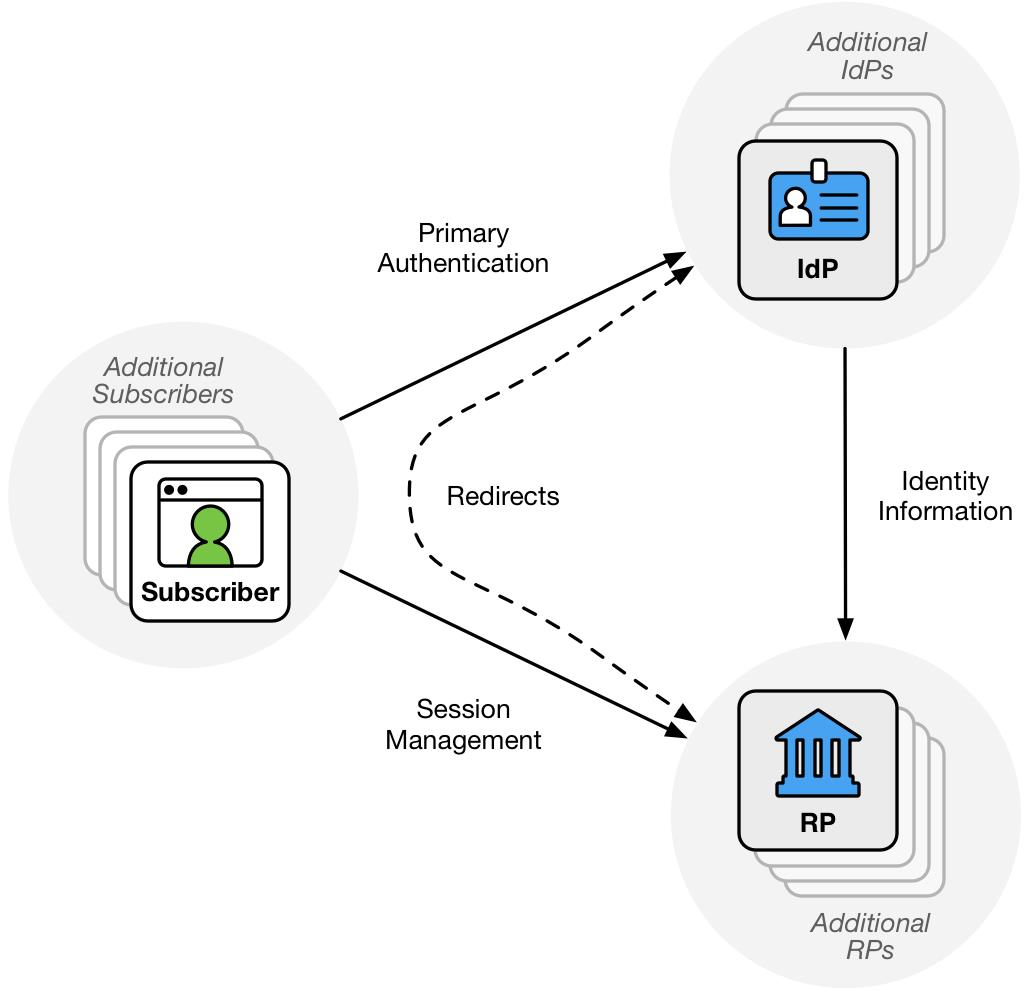
\includegraphics[width=0.8\textwidth]{images/federation}
		\caption[Federation]{Federation}
		\label{fig:federation}
	\end{figure}
	
	
	The user or subscriber is usually associated with a real user, and their identity is represented by a set of attributes. A single user can be associated with multiple identities. A service/resource provider is responsible for making an authorization decision based on authentication assertion and the attributes derived from it. Many of the service providers implement their identity management, but in federated systems, the identity management is outsourced to the identity provider. An identity provider can be either a stand-alone service or be a part of the service provider. The responsibility of the IdP is it to authenticate the user, issuing authentication assertions, manage identities whereas the IdP has the right to create, update, release and delete attributes associated with the identity [cf. (\cite{Birell:2013:FIMS})]. 
	
	
	The 'Digital Identity Guidelines' by Grassi, Garcia \& L. (2017) claim that identity federation is preferred over some siloed identity solution that each serve a single agency or Relying Party (RPs). Furthermore The 'Digital Identity Guidelines' by Grassi, Garcia \& L. (2017), lists specific benefits that come with using federated architectures, as can be examined before. 
	
	\begin{itemize}
		\item Enhanced user experience. For example, an individual can be identity proofed once and reuse the issued credential at multiple RPs. 
		\item Cost reduction to both the user (reduction in authenticators) and the agency (reduction in information technology infrastructure). 
		\item Data minimization as agencies do not need to pay for collection, storage, disposal, and compliance activities related to storing personal information. 
		\item Pseudonymous attribute assertions as agencies can request a minimized set of attributes to include claims or to fulfill service delivery. 
		\item Mission enablement as agencies can focus on the mission, rather than the business of identity management.
	\end{itemize}
	
	Essentially switching to a federated identity solution should help to reduce the management burden that comes from managing multiple accounts and can lead to potential points of failure.  Furthermore, users are giving control over their attributes dissemination which leads to privacy violations and identity theft. Most of the existing identity federation solution focuses on the individual system, each of which focuses on one of three general types of functionality - SSO, federated identity or anonymous credentials. The SSO system can issue authentication assertion to multiple service providers. Examples for SSO are Passport, OpenID or Shibboleth. Federated identity systems are focused on managing multiple identities for a single user. Examples for federated identity are Project Liberty (http://projectliberty.org), Higgins (www.eclipse.org/higgins), PRIME (www.prime-project.eu), CardSpace, and
	Client-Side Federation. Anonymous credentials systems provide authentication assertions while not revealing the user's identity to a service provider. Examples include Idemix, U-Prove, and P-IMS [cf. (\cite{Birell:2013:FIMS}), (\cite{Boyed:2012:GSOA}), (\cite{NIST:2017:DIG})].
		
		\subsection{Single Sign-On}
		\label{singlesignon}	The focus of this thesis is on mobile SSO solutions. SSO aims to design an authentication system that serves the interests of the user as well as the interests of the service provider. Whereas the user prefers a simple process, the service provider requires a complicated authentication procedure. Ironically trying to make the authentication procedure more save often leads to weakening the whole system due to the user always finding new ways to bypass it. An example mentioned before for this conundrum, is password fatigue. Another challenge that SSO is trying to tackle is that standard web authentication solutions that require the user to login with a password, only authenticate the user and are not capable of providing access control or revealing additional information about the user. Most SSO solutions, therefore, try to combine the authentication process and authorization [cf. (\cite{Prochazka:2010:UCA})].
		
		The paper 'Taxonomy of Single Sign-On System' by Pashalidis \& Mitchell (2003) identifies four generic architectures for SSO systems. An SSO system has to authenticate a user to an Service Provider (SP). Because authentication also implies identification, SSO systems have to incorporate the lifecycle management of identifiers that can take various forms. The paper distinguishes between two main types of SSO systems. The first type is ‘pseudo-SSO’ and the second type is ‘true SSO’. Typical pseudo-SSO are providing automatic authentication for all SP specific authentication methods after the user initially authenticated with the pseudo-SSO component, which is called primary authentication. The responsibility of a pseudo-SSO service is to manage all identities. A user may have multiple SSO identities for a single SP, but in principle, one SSO identity corresponds to one SP. Compared to the pseudo-SSO system in a true-SSO system, the user has to initially authenticate with the Authentication Service Provider (ASP) that is required to have an established relationship with all SPs. The relationship between the ASP and the SP has to be trustworthy. Key functionality of the true-SSO service is that the only authentication that includes the user occurs between the user and the ASP. The SP will get notified of the authentication status, including information about the identity of the user, with so-called authentication assertions. The categorization of SSO architectures can be further distinguished by the location of the ASP/pseudo-SSO component. This component can be either local to the user platform or offered as a third-party service also called SSO-proxy. This further categorization leads Pashalidis \& Mitchell (2003) to the four generic architectures mentioned above Local pseudo-SSO systems, Proxy-based pseudo-SSO systems, Local true SSO systems and Proxy-based true SSO systems  [cf. (\cite{Pashalidis:2003:10.1007/3-540-45067-X_22})].
		
		When opting for a particular SSO architecture, one has to consider the strength and weaknesses of each system carefully. The paper, therefore, analyses the four generic architectures regarding pseudonymity and unlinkability, anonymous network access, support for user mobility, deployment costs, maintenance costs, running cost and trust relationships. Pseudonymity and unlinkability refer to the fact that the user providers sensible information that needs to be protected and it should not be possible to correlate distinct identities of the same user and personal information, and potential properties should not be linked to the user. The unlinkability cannot be guaranteed for pseudo-SSO because the identities for the SSO are SP specific. To improve unlinkability   Pashalidis \& Mitchell (2003), suggest to use an ‘anonymizing proxy’. For local SSO system additionally services are needed to implement a anonymizing proxy. In proxy-based SSO systems the anonymizing proxy can be integrated. User mobility is supported for proxy-based SSO, for locale SSO there need to be further services in place. The deployment cost is lower for pseudo-SSO systems than for true-SSO systems. However, the maintenance cost is higher because if any SPs change the whole logic of the pseudo-SSO system has to change. The running cost of pseudo-SSO is likely to be lower than for true-SSO systems. For the pseudo-SSO systems, the trust relationship between users and SP may be dynamically changing depending on the implementation, for true-SSO the trust relationship is established between ASP and SPs and is always consistent. Generally speaking are pseudo-SSO systems are more suitable for a closed system where identity management is just for managing the life cycle of remaining credentials. For an open system, it is not enough to maintain credentials. Appropriate privacy protection services and privacy-aware identity management schemes should be therefore integrated with true SSO schemes [cf. (\cite{Pashalidis:2003:10.1007/3-540-45067-X_22})]. 
			
		Therefore two very popular assertion technologies are discussed: Shibboleth (SAML) and OpenID Connect. Those technologies are not the only possible SSO assertion technologies however, they represent the most commonly used federated identity systems. According to Lynch (2011), two SSO solutions gained broad acceptance. The two SSO solutions are SAML-based federations using SOAP with focus on large enterprises, governments and educational networks and the Web Authorization Protocol is a combination of the Protocols OpenID and OAuth. SAML federations have been customized to address the security concerns of those institutions that typically have a large user base, significantly protected resources, complex authorization patterns and data and services spread across multiple domains. However, in a Web 2.0 world, the SAML solutions where seen as too rigid and too severe to maintain; a lightweight SSO was needed, therefore the Web Authorization Protocol was designed. The approach of this protocol is taking advantage of the lightweight RESTful APIs which are reusing the existing HTTP architecture features and the JavaScript Object Notation (JSON) [cf. (\cite{Lynch:2017:IIG})].
			
		\paragraph{SAML}
		\label{SAML}
		One of the well-known solutions based on Security Assertion Markup Language version 2 (SAML2) is Shibboleth. Shibboleth is one of the leading middlewares for building identity federations in a higher education sphere. It offers authentication, authorization and attribute assertion between entities. Procházka, Kouřil \& Matyska (2010), identifies the following entities Identity Provider (IdP), Service Provider (SP), Discovery Service, Metadata Operator and Federation Operator  [cf. (\cite{Prochazka:2010:UCA})].
		
		The discovery service is used to find the users organization IdP. The IdP defines an attribute release policy and releases different sets of the user's attributes to different SPs. Users are only able to agree or disagree with the whole set of attributes because the decision comes from the IdP. When the user tries to log on, to a service of a Service Provider, the user gets redirected to a page where an IdP previously found by the Discovery Service can be chosen. If an SP wants to provide their service to multiple federations it has to negotiate policy and technical detail with each federation operator. The federation operator manages the federation policies and introduces SPs and IdPs. Furthermore, the federations operator has to maintain and manage the information about all entities in a federation which is contained in the Metadata. A problem with this architecture is that the SP has to keep track of changes of the technical specification of various federation operators to maintain the configuration for each federation operator. A solution would be a significant federation registration, but this is indeed not possible because of technical and administrative severity and political will. This solution is also somewhat misleading for users since they have to maintain multiple credentials, select from multiple identifiers and so on. According to Procházka, Kouřil \& Matyska (2010) Shibboleth is too restrictive, a solution with a centrally managed point of IdPs and SPs is preferred. Also, users should not have to deal with redundant accounts [cf. (\cite{Prochazka:2010:UCA})].		
		
		\paragraph{OAuth and OpenID Connect}
		\label{OAuthAndOpenID}
		The second solution that is introduced is OAuth 2.0 with OpenID Connect.	OAuth 2.0 is a protocol that is used for access control. OAuth 2.0 is the newest version of  OAuth. Compared to the previous version OAuth 1.0a, HTTPS is used for all request, and the complicated signature process of tokens was replaced. Additionally, complexity was reduced, and the usage is much simpler than in the first version. The new version OAuth 2.0 is not compatible with older versions [cf.  (\cite{LeBlanc:2011:SocialApplications})].
		
		The protocol adds an authorization layer – separating the Client from the Resource Owner. 
		The Client is not bound to any particular implementation characteristics and can make requests to protected resources on behalf of the resource owner. The OAuth 2.0 specification distinguishes between two Client Types, Confidential Clients, and Public Clients. Confidential clients are capable of maintaining the confidentiality and public clients are incapable of maintaining confidentiality [cf. (\cite{Hardt:2012:OAuth2}, p.6-14)].
		
		The Resource Owner is a role according to Sakimura et al. (2014) which can grant access to a protected resource also referred to as end-user, if the resource owner is a person. Furthermore, scopes are used to specify to which resources the resource owner wants to grant access. Requests which are sent to an authorization endpoint include scopes that can be mandatory or optional parameters. Declaring the scopes is up to the provider. An access token is used to gain access instead of the resource owner’s credentials [cf. (\cite{Sakimura:2014:OpenIDConnect}, p.6)]. 
		
			\begin{figure}[h]
			\centering
			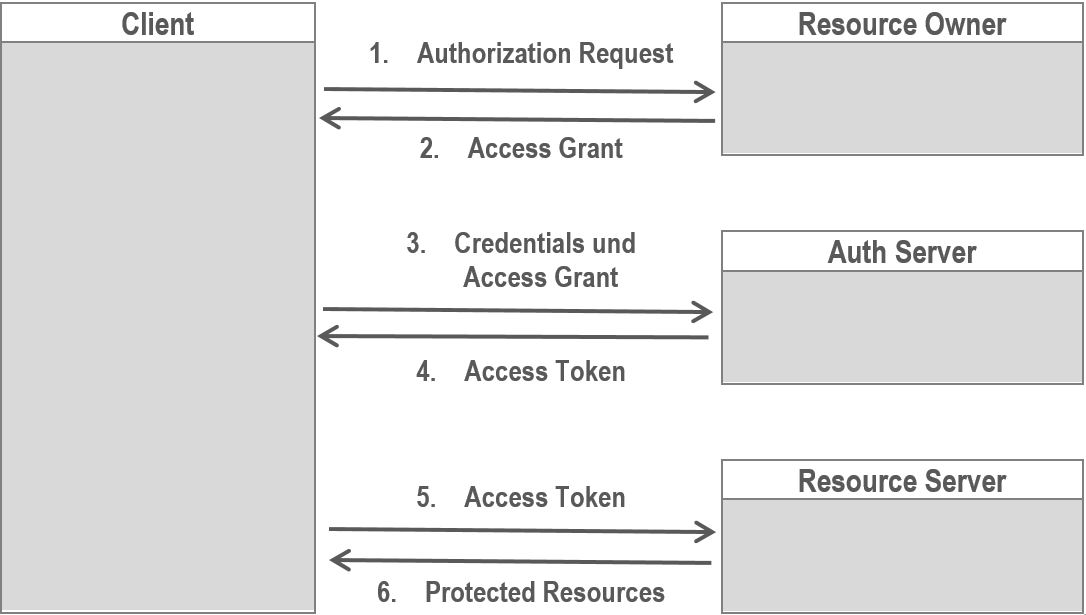
\includegraphics[width=0.8\linewidth]{images/oaut-process2}
			\caption{OAuth Authorization Process (\cite{LeBlanc:2011:SocialApplications}, p. 353)}
			\label{fig:oaut-process2}
		\end{figure}
		
		Access Tokens are issued by an Authorization Server and can be used by the Client to gain access to protected resources hosted by the resource server. The Authorization Server is responsible for issuing the access token and may be the same as the Resource Server. In literature, different terms are used do describe what an identity server does. Among these are Security Token Service, Identity Provider, Authorization Server and IP-STS. OAuth 2.0 uses a token service, which centralizes this logic and reduces complexity for the Client and the APIs [cf. (\cite{Sakimura:2014:OpenIDConnect}, p. 6), (\cite{Brock:2018:ID4}), (\cite{Boyd:2012:GSOAuth})]
		
		A typical request of a Client to access a resource on the Resource Server includes some requests. In the end, the Client should be able to access the protected resource. The process is shown in figure \ref{fig:oaut-process2}.
			
		In the first two steps, the Client redirects the user to the Resource Owner, to give the Client permission to access the protected resources. The user is then redirected to the callback location which is included in the original request and adds a verification code which confirms that the Client is entitled to access the requested resource. After the redirection to the callback location, the Client sends a request with the verification code to the Authorization Server. If the request is a success, the Authorization Server replies in step four with an access token and eventually a refresh token. With the received access token the client can now make signed requests to the resource server and receive in return protected resources as shown in step five and six inf figure~\ref{fig:oaut-process2} [cf. (\cite{LeBlanc:2011:SocialApplications}, p. 353)]
		
		
		OpenID Connect and OAuth 2.0 seem very similar but OpenID Connect is a framework built on top of OAuth 2.0. Together they focus on authentication and access control in a way that is suitable for modern applications. OpenID Connect can verify the identity of an End-User and obtain basic profile information about the user. It uses Claims to communicate information to the end-user [cf. (\cite{Sakimura:2014:OpenIDConnect})]
		
		OpenID Connect performs authentication and determines if the user is already logged on or to log on the user. The result is an authentication token which is returned to the user. A precondition of OpenID Connect is that the client, as well as the user, have to trust the IdP. The functions of the IdP are the same as in OAuth. The reason for that is that the newest version of OpenID is implemented on top of OAuth and extends the authentication process of OAuth  [cf. (\cite{Sakimura:2014:OpenIDConnect}), (\cite{Boyd:2012:GSOAuth}, p. 51)]
		
		\begin{figure}[h]
			\centering
			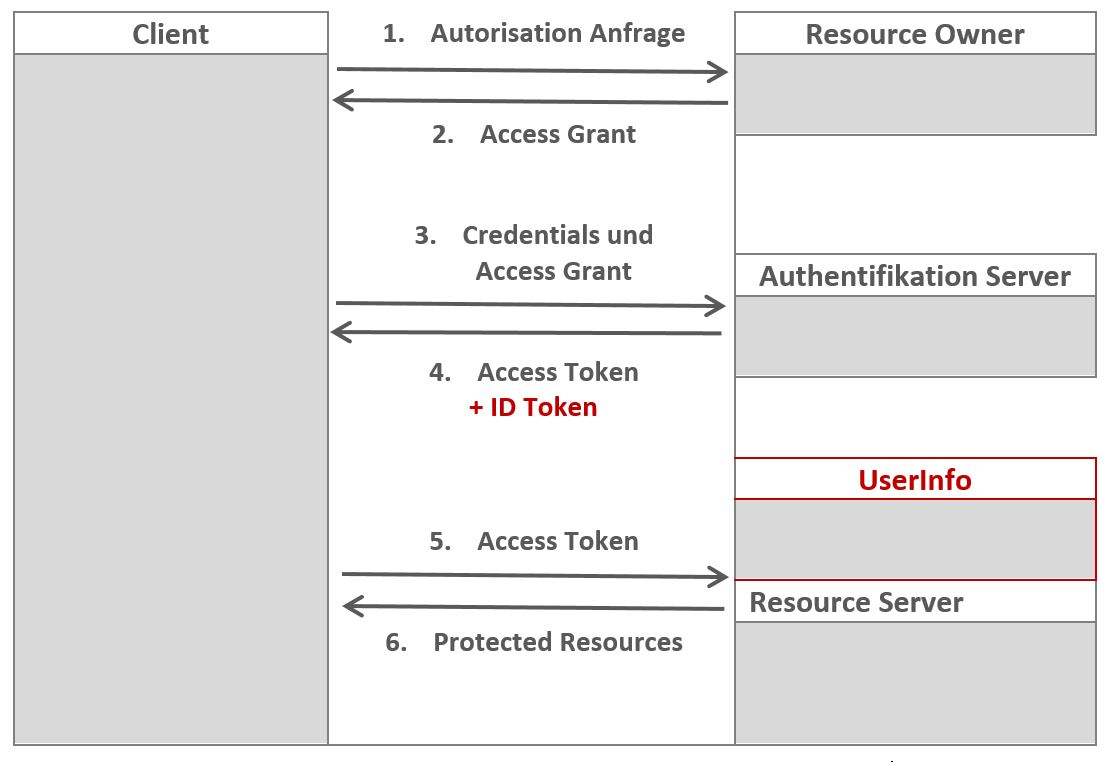
\includegraphics[width=0.8\linewidth]{images/openid-process}
			\caption{OAuth 2.0 and OpenID Connect (\cite{Lodderstedt:2014:OpenID})}
			\label{fig:openid-process}
		\end{figure}
		
		
		In figure~\ref{fig:openid-process} the added element of the OpenID Connect standard is marked with red. In order to implement the OpenID Connect Standard, the Client has to request the scope 'openid'. After the request, the progress is similar to the transitional OAuth authentication process, but when it comes to returning of the access token, an additional ID Token is returned. This ID Token holds information about the user and the authentication. The only purpose of the ID Token is to log in the client. The only thing left after this is for the client to verify the ID Token [cf. (\cite{Lodderstedt:2014:OpenID})]. 
		
		The ID Token is specified by Sakimura et al. (2014) as a JWT compared to OAuth were the type of token is irrelevant. The token is signed and has some particular claims. Further individual claims could also be added to the ID token. The ID token has claims that are required for the authentication process. Also, standard claims can be added which are predefined by OpenID Connect. Those claims could also be requested from UserInfo Endpoint shown as an additional endpoint in the figure~\ref{fig:openid-process}. The user info endpoint offers an API where additional user info can be requested [cf. (\cite{Sakimura:2014:OpenIDConnect})].
		
		Lodderstedt (2014), says that OpenID Connect is a contemporary advancement from protocols like SAML. The protocol considers the ongoing development of web services and mobile applications. Furthermore, the implementation of the protocol is quite easy and uses little HTTP requests with minimal cryptographic overhead to accomplish a complete login process [cf. (\cite{Lodderstedt:2014:OpenID})]. 
		
		
		
		
		
		
		Sakimura et al. (2014) defines three different way authentication can flow:
		
		
		\begin{enumerate}
			\item \textbf{Authorization Code Flow}  - The Authorization Code Flow returns an Authentification Code which can be used to be exchanged for an id\_token or an access\_token. The Authorization Code is used for Clients that can maintain a secret securely between themselves and the Authorization Server. Typically this approach is used for server-to-server communication when no interactive user is present. In this thesis, the focus is on user interaction [cf. (\cite{Sakimura:2014:OpenIDConnect}, p. 10)]
			
			To use the Authorization Code Flow according to Sakimura et al. (2014) the following request\_type indicates a Authorization Code Flow:
			\begin{itemize}
				\item	code: The response includes an Authorization Code. 
			\end{itemize}
			
			\item \textbf{Implicit Code Flow} - In the Implicit Code Flow the access token and the id token are directly returned to the Client. This behavior may expose information to the end-user or anyone who has access to the end-user’s Agent. Tokens are only returned from the Token Endpoint; the Authorization Endpoints is not used. Unlike the Authorization Code Flow where the separate request is used for authorization and authentification, here the Client will receive the access token as a result of the authentification which also means that there is no refresh token.  This flow is used for Clients who are implemented in a browser using scripting language [cf. (\cite{Sakimura:2014:OpenIDConnect}, p. 20), (\cite{Hardt:2012:OAuth2})]
			
			According to Sakimura et al. (2014), the following request\_types indicate an Implicit Code Flow:
			\begin{itemize}
				\item	id\_token: The response must include the parameter id\_token. The response does not include an Authorization Code, Access Token, or Access Token Type. 
				\item  id\_token token: The response includes an Access Token, an Access Token Type and an id\_token.
			\end{itemize}
			
			\item \textbf{Hybrid Code Flow} - In the hybrid code flow, tokens are returned from the Authorization Endpoint, and others are returned from the Token Endpoint. The Token Server will return not only the id token but also the code. The Client then has to use the code in order to gain the access token through a back channel call which means there is an additional round trip compared to the Implicit Code Flow. Using the code to receive the access token should minimize the risk of exposing the access token [cf. (\cite{Sakimura:2014:OpenIDConnect})].
			
			To use the Hybrid Code Flow according to Sakimura et al. (2014) the following request\_types indicate a Hybrid Code Flow:
			\begin{itemize}
				\item	code id\_token: The response includes an Authorization Code and an id\_token.
				\item  code id\_token token: The response includes an Authorization Code, an Access Token, an Access Token Type and an id\_token. 
			\end{itemize} 
			
		\end{enumerate}
		
		Both OpenID Connect and SAML SSO solution involve different layers of communication and exchange credentials using HTTP redirection and Javascript which leads to vulnerabilities. Vulnerabilities include Cross-Site Request Forgery and Cross Site Scripting. The authentication process for SSO solution includes redirects which can be exploited by attackers. As the SP redirects the User to the IdP, an attacker could intervene and send the user to a fake IdP. If the user does not recognize to swap from the real IdP to the fake IDP, the attacker ends up with the user's credentials. This problem is called a malicious IdP, also known as “phishing” and a very well-known attack against SSO. Another problem that a federation SSO system could be facing is a malicious RP or SP. After a user successfully authenticates on the IdP site, the user is redirected back to the SP with a link. An attacker obtains a link with methods like sniffing and uses the link to get logged into the SP as the User [cf. (\cite{Xu:2015:SPSSO})].
		
		OpenID Connect and SAML both provide SSO solutions. However, there is the view of the differences between the two protocols. First, in SAM an SP and OpenID, the RP redirects the user to the IdP. The assertions distinguish themselves by the markup language which is used. SAML uses a signed XML document and OpenID uses a signed JSON document. The JSON format makes tokens easier to parse with Javascript. Furthermore, OpenID Connect was designed to work with the web while SAML was readjusted to work on top of the web 	[cf. (\cite{Schwartz:2016:OAuthVsSamel}), (\cite{KeyCloack})].
		
		Schwartz (2016), suggest using OpenID Connect for mobile applications, API's and any new applications in general. SAML is just suggested for applications that already use SAML. Nevertheless, KeyCloack (2018) expresses that choosing between this SSO protocol is not straightforward. Although they recommend the use of OpenID Connect, they notice the gradual development of OpenID Connect and how more and more features are implemented that SAML had for years. Therefore some people tend to pick SAML over OIDC, based on the perception that it is more mature [cf. (\cite{Schwartz:2016:OAuthVsSamel}), (\cite{KeyCloack})].
		

\chapterend
  %%%%%%%%%%%%%%%%%%%%%%%%%%%%%%%%%%%%%%%%%%%%%%%%%%%%%%%%%%%%%%%%%%%%%%%%%%%%%
\chapter{Analysis of Identity Management}\label{chap:analysis}
%%%%%%%%%%%%%%%%%%%%%%%%%%%%%%%%%%%%%%%%%%%%%%%%%%%%%%%%%%%%%%%%%%%%%%%%%%%%%
\chapterstart

This chapter consists of two parts: the use case and a risk assessment. In the first part a use case is described. The use case tries to picture a typical scenario that requires thoughtful consideration of authentication and authorization technologies depending on the requirements of the use case. Based on the use case a minor risk assessment is done. The risk assessment takes typical threats emerging from authentication and authorization and establishes a risk profile. This risk profile should help to choose an appropriate level of assurance for identity proofing, authentication and federation. 

\section{Use Case}
\label{usecase}
This use case is based on an similar use case of the company "ACP Business Applications" where I am currently employed. This should allow the reader to get a better understanding of the circumstances that led to the design of a federated authentication solution. 

The use case features a medium to large company with up to 1000 employees. The mission of the company is to provide a network and analyzing toolset which allows the customer of the product suite to improve security within his network and keep an overview of potential security risks. Previously the customers received monthly reports about their current state of the network. Each of the products and tools resulted in a separate report which was sent via e-mail. To modernize the approach, the reports should be replaced by a modern single-page application that could be accessed by customers and by employees for administrative reasons. In this example, we call the solution 'Security Assessment Portal.' The Security Assessment Portal should give the customers an overview of current products and the performance of the network. An example of the toolset could be E-Mail-Filtering. The example will be focused on an E-Mail-Filtering-Report and the data which is exposed via the report. It is very important to have a good overview of the data that is used within the application in order to establish appropriate security controls. The Email-Filtering-Report will display a chart per domain. The chart includes data about the amount of e-mails which were blocked, received or carried a virus. 

The company already has a particular set of internal applications that are used by the employees within the company network. The company internally uses active directory for authorization on local machines. All applications until now are accessible within the companies network and are using windows authentication. The application should be accessible by employees as well as customers whereas customers should not receive access to the company network. The data of the customers is sensitive and therefore worth protecting. However it should be kept in mind that because of the sensitive data, certain customer do not want to authenticate with an external provider. The application should be hosted within the company and a solution for customers to access the application from outside is needed. The company needs an authentication solution that meets all the outlined requirements while balancing usability and security. 

The description gives an overview of the company and the expectations for the new application. This leads to the following requirements for the system architecture:

\begin{itemize}
	\item Access from outside the company network is enabled
	\item Application is secured with accounts
	\item Accounts should be managed within the company
	\item Only authenticated users have access to secure contents
	\item Single sign-on for convenience
	\item API for data access
	\item Data can be hosted within the company
	\item The application should be a light weighted Angular solution
\end{itemize} 

The application and its requirements are taken into account in the risk assessment conducted in the next section \ref{riskassessment}. The risk assessment should lead to an better understanding which security measurements are needed for this use case. 

\section{Risk Assessment}
\label{riskassessment}
Risk Assessment is one of the essential elements when it comes to managing risks of an organization. The aim of risk assessment is it to identify, estimate, and prioritize risk to operations, assets, individuals, other organizations and use of the information system. The main task of a risk assessment is to help making decisions on how to respond to certain risk. The steps to a risk assessment are identifying potential threats, internal and external vulnerabilities, the impact to organizations given the potential for threats exploiting vulnerabilities and the likelihood of that harm to occur. There are three tiers according to the 'Guide for Conducting Risk Assessment by NIST (2012) in risk management:

\begin{itemize}
	\item Tier 1 - organizational level
	\item Tier 2 - mission/business process level
	\item Tier 3 - information system level
\end{itemize}

The first two tiers are focusing on risks related to organizational governance and management activities, mission/business processes, enterprise architecture or the funding of information security programs. The third tier focuses more on how to implement a risk management framework successfully [cf. (\cite{NIST:2012:GCRA}, p.1)]. 

The result of the risk assessment should state which assurance levels are appropriate. The available assurance levels are identity proofing assurance level, authentication assurance level and the federate assurance level. Identity proofing assurance level describes the robustness of the process to determine the identity of an individual and should help to avoid identity proofing errors. To determine the robustness of the authentication process and the binding of an authenticator and a specific individual's identifier the authentication assurance level is used. Furthermore choosing an appropriate authentication assurance level should help to avoid authentication errors. The last one of the assurance level is the federated assurance level which is optional since not all identity systems need a federated identity solution. The federated assurance level determines the robustness of the assertion protocol the federation uses to communicate authentication and attribute information and should help to avoid federation errors. All of the assurance levels a described in more detail in the sections \ref{identityProofing} Identity Proofing, \ref{authentication} Authentication and \ref{assertion} Assertion [cf. (\cite{NIST:2017:DIG}, p. 19)]. 

To determine assurance levels one needs to identify the potential risk and which measures exist to minimize the impact of those risks. Two factors are crucial for this task. The first factor is the potential harm or impact, and the second the likelihood of such harm or impact [cf. (\cite{Bolton:2003:EAuth}, pp. 3)]. Bolton (2003), splits harm and impact into these categories:

\begin{itemize}
	\item Inconvenience, distress, or damage to standing or reputation
	\item Financial loss or agency liability
	\item Harm to agency programs or public interests
	\item Unauthorized release of sensitive information
	\item Personal safety
	\item Civil or criminal violations
\end{itemize}

Assurance levels are determined by assessing the potential impact of these categories. The 'Federal Information Processing Standard Publication' by NIST (2004), defines three levels of potential impact concerning security objectives confidentiality, integrity, and availability. Those levels of potential impacts can affect in case of a security breach either the organization or individuals. The levels of impact defined in 'Federal Information Processing Standard Publication' by NIST (2004) are:

\begin{itemize}
	\item Low
	\item Moderate
	\item High
\end{itemize}


If the level is low the loss of confidentiality, integrity or availability has a limited effect. This can mean for example minor damage to organizational assets, short-term inconvenience, short-term distress, short-term embarrassment, limited reveal of personal or sensitive information to unauthorized parties with minor impact, minor financial loss, risk of civil or criminal violation which would not ordinary be subject to enforcement efforts, minor harm to individuals or the capability of the company to fulfill their mission is degraded. If the level of impact is moderate the effects of loss of confidentiality, integrity or availability are serious. Impacts can be significant damage to organizational assets, significant financial loss, serious short-term or limited long-term inconvenience,  serious short-term or limited long-term distress,  serious short-term or limited long-term damage to standing reputation, release of personal or sensitive information to unauthorized parties with moderate impact, risk of civil or criminal violations which may be subject to enforcement efforts, significant harm to individuals or significant degradation of mission fulfillment. The last level of potential impact is high, meaning that the effects can be severe or catastrophic. This means for example major damage to organizational assets, major financial loss, severe or serious long-term inconvenience, severe or serious long-term distress, severe or serious long-term damage to standing reputation, release of personal or sensitive information to unauthorized parties with high impact, risk of civil or criminal violation with special importance to enforcement programs, harm to individuals involving loss of life or serious life-threatening injuries and loss of capability to fulfill the mission [cf. (\cite{NIST:2004:FIOPS}, pp. 6), (\cite{NIST:2017:DIG}, pp. 21)].


The results of the risk assessment are needed to determine the minimum LOA. Once the risk assessment is complete the risk assessment impact profile can then be compared to the impact profiles associated with each assurance level. The table \ref{tab:maxImpacts} can help to determine the required assurance level by finding the lowest level whose impact profile meets or exceeds the potential impact for every category analyzed in the risk assessment [cf. (\cite{NIST:2017:DIG}, p. 25)].

\begin{table}[h]
	\centering
	\begingroup
	\setlength{\tabcolsep}{10pt} % Default value: 6pt
	\renewcommand{\arraystretch}{1.5} % 
	\begin{tabular}{lccc}
		\hline
		\rowcolor[HTML]{656565} 
		{\color[HTML]{FFFFFF} }                                                                                                     & \multicolumn{3}{c}{\cellcolor[HTML]{656565}{\color[HTML]{FFFFFF} Assurance Level}}                  \\ \hline
		\multicolumn{1}{|c|}{\textbf{Impact Categories}}                                                                            & \multicolumn{1}{c|}{\textbf{1}} & \multicolumn{1}{c|}{\textbf{2}} & \multicolumn{1}{c|}{\textbf{3}} \\ \hline
		\multicolumn{1}{|l|}{\begin{tabular}[c]{@{}l@{}}Inconvenience, distress or damage to\\ standing or reputation\end{tabular}} & \multicolumn{1}{c|}{Low}        & \multicolumn{1}{c|}{Mod}        & \multicolumn{1}{c|}{High}       \\ \hline
		\multicolumn{1}{|l|}{Financial loss or agency liability}                                                                    & \multicolumn{1}{c|}{Low}        & \multicolumn{1}{c|}{Mod}        & \multicolumn{1}{c|}{High}       \\ \hline
		\multicolumn{1}{|l|}{Harm to agency programs or public intrests}                                                            & \multicolumn{1}{c|}{N/A}        & \multicolumn{1}{c|}{Low/Mod}    & \multicolumn{1}{c|}{High}       \\ \hline
		\multicolumn{1}{|l|}{Unauthorized release of sensitive information}                                                         & \multicolumn{1}{c|}{N/A}        & \multicolumn{1}{c|}{Low/Mod}    & \multicolumn{1}{c|}{High}       \\ \hline
		\multicolumn{1}{|l|}{Personal safty}                                                                                        & \multicolumn{1}{c|}{N/A}        & \multicolumn{1}{c|}{Low}        & \multicolumn{1}{c|}{Mod/High}   \\ \hline
		\multicolumn{1}{|l|}{Civil or criminal violation}                                                                           & \multicolumn{1}{c|}{N/A}        & \multicolumn{1}{c|}{Low/Mod}    & \multicolumn{1}{c|}{High}       \\ \hline
	\end{tabular}
	\endgroup
	\caption{Maximum Potential Impacts for Each Assurance Level (\cite{NIST:2017:DIG}, p. 25)} \label{tab:maxImpacts}
\end{table}

When analyzing the risk, it should be considered that there could be more than one error and multiple parties could be involved in the process. Furthermore, the potential impacts description often include relative terms like 'minor' and 'serious' which meaning will depend on the context. Over time and with experience the meaning of these relative terms becomes more definite [cf. (\cite{NIST:2017:DIG}, p. 26)].

One of the most useful documents is NIST's 'Guide for Conducting Security Risk assessment'. The guide follows activities related to NIST'S guide of 'Risk Management Framework' which can be either applied to new or legacy information systems. Typically a risk assessment is a very complex task that takes much time and many external sources to be representative, for example expert opinions. If put together correctly one should end up with a Risk Management Framework (RMF). An RMF provides a process that integrates security and risk management activities into the system development life cycle. The system can be applied to both new and legacy systems. 'Risk Management' by NIST (2018) defines 6 Steps in this RMF. The steps include the categorization of the information system, selection of baseline security controls, implementation of security controls, assessment of the security controls, authorize information system operation based on the determination of risk and monitoring security controls. Many industrial standard risk assessment methods across a wide array of fields and industries are based on these guides.  In this practical part, an initial risk assessment is done which should provide a general insight on how to do a risk assessment. The guide to success of a real-life risk assessment is documentation, review, and improvement.  However, since a full RMF is out of scope, a scaled down version that is distinctive of digital identity risk management is conducted  [cf. (\cite{NIST:2018:RMF})].


To prepare for a risk assessment, it helps to identify the purpose, scope, assumptions, and constraints beforehand. The purpose of this risk assessment is to make authorization-related decisions and conducting an initial assessment to identify potential threats, internal and external vulnerabilities which impact the organizations. The scope addresses the 3 Tier -  information system level with a focal point on the risk assessment of a single sign-on federation system. Furthermore, the scope is defined by the result expected from the risk assessment. In this risk assessment, the result should be an authentication and authorization solution for a specific use case. The assessment result should usually be reevaluated after the initial draft. [cf. (\cite{NIST:2012:GCRA}, pp. 24)].

Before starting with the risk assessment a risk model has to be chosen. The model can be translated into risk factors which then can be assessed; these risk factors consist of threat, vulnerability, impact, likelihood and predisposing conditions.  A threat is a circumstance with the potential to impact the organization. Threat events are caused by threat sources. Threat sources that should be considered in the model can address broad threat sources or particular threat sources. Potential threat sources can be adversarial like Insider, Outsider, Trusted Insider, Privileged Insider, Customer, or Competitor. A thread source can also be accidental like User, Privileged User/Administrator or structural like IT-Equipment (Storage, Communication, Processing), Environmental (Temperature/Humidity, Power Supply) or Natural (Fire, Bombing, Earthquake, Sunspots). These potential sources can then cause threat events which can be expressed very general or can also be very specific. Which threat are considered depend highly on the company. A company might choose to only consider previously observed events or all possible events. Examples of potential threat sources are cause integrity loss by injecting false but believable data into organizational information systems, obtain unauthorized access, obtain sensitive data/information from publicly accessible information systems, cause disclosure of critical and/or sensitive information by authorized users, conduct externally-based session hijacking, conduct simple Denial of Service (DoS) attack, craft phishing attacks and so on. The likelihood is a weighted risk factor based on the probability that a given threat is capable of exploring a given vulnerability. A vulnerability is an existing weakness in an information system, system security procedures, internal controls, or implementation that could be exploited by a threat source. Most vulnerabilities are caused by unimplemented or not correctly implemented security controls. Some recommended security controls are described in 'Recommended Security Controls for Federal Information Systems and Organizations'. The implementation of appropriate security controls is an important task that can have a major impact on the operations and assets of a company. Security controls are used to protect the confidentiality, integrity and availability of a system and it's information. Examples are Identifier Management, Authenticator Management or Authenticator Feedback. Closely related to vulnerabilities is a predisposed condition which is a condition within a company which affects the likelihood that threat events once initiated, result in adverse impact on the organization like the involvement of PII. The consequences that a successfully exploited vulnerability by a threat source has, is then described by the impact  [cf. (\cite{NIST:2012:GCRA}, pp. 17, pp. 35, pp. 70), (\cite{NIST:2017:SecurityNPrivacyControls})].

Last but not least before stating a risk assessment based on a risk model, an analytic approach and an assessment approach should be considered. The assessment approach can be quantitative, qualitative or semi-quantitative each of the factors including three assessment scales with different corresponding representations. A quantitative assessment is based on the use of numbers whereas the qualitative assessment typically uses nonnumerical categories or levels like very low, low, moderate, high, very high. Finally, semi-quantitative assessment is a combination of a quantitative and a qualitative assessment using bins, scales or representative numbers. For low impact information systems, the qualitative values are used while for moderate-and high-impact systems; the most granular semi-quantitative values are used. The analysis approach is either threat-oriented, asset/impact-oriented or vulnerability-oriented. With the analysis approach the starting point of the risk assessment can be chosen. The risk assessment starting point can either be based on existing vulnerabilities or assets in the company or possible threats  [cf. (\cite{NIST:2012:GCRA}, pp. 17)].

Based on this knowledge a few examples considering the use case above where conducted. Based on the remarks above and on an example from Hudson (2015) the following steps were followed  'Identify Threat', 'Identify Vulnerability', 'Current Controls', 'Likelihood of Impact', 'Effect of Impact' and 'Risk Determination'. Since it is an initial risk assessment, there are no 'Current Controls'. Therefore, this step is left out. The 'Likelihood of Impact' can be assigned a value from low to high whereas high means it is very likely that a vulnerability is exploited by a threat. The lowest value of 'Likelihood of Impact' is 0.1, and the highest is 1. The 'Effect of the Impact' is assigned a value between 0 to 100. A low 'Effect of Impact' means that the consequences are low and high 'Effect of Impact' means that the consequences are severe. Next to the 'Effect of Impact' of each analysis the associated impact categories are pointed out in order to make it easier to compare the results to the table \ref{tab:maxImpacts}. To determine to the overall risk of a threat, the 'Likelihood' is multiplied with the 'Impact' (Likelihood x Impact) resulting in the risk levels below [cf. (\cite{Hudson:2015:SecurityRisk})]. 

\begin{itemize}
	\item Low =     0-33
	\item Medium = 34-66
	\item High =   67-100
\end{itemize}

Since this analysis is about identity proofing, authentication and federation errors a few threats were chosen to be analyzed with the risk assessment. It should be noted that this does not represent a complete risk assessment since there are more factors to be considered. The risk analysis sees outsiders who want to harm the company and users and identifies them as potential threat sources. 

\paragraph{Identity Proofing Risk 1}

\begin{enumerate}
	\item Technical Threat: An attacker successfully proofs as someone else
	\item Vulnerability: Phishing over unencrypted network communication
	\item Likelihood: 0.5
	\item Impact: 80 (Inconvenience, distress or damage to standing reputation)
	\item \textbf{Risk Determination}: 0.5 x 80 = 40 (Medium Risk) 
\end{enumerate}
\pagebreak[4]

\paragraph{Identity Proofing Risk 2}
\begin{enumerate}
	\item Technical Threat: Collecting and securely storing more information about a person that is required to successfully provide the digital service
	\item Vulnerability: Identity Provider is collecting more information than needed from the user on login. Users might not trust the application or not use it
	\item Likelihood: 0.8
	\item Impact: 30  (Unauthorized release of sensitive information)
	\item \textbf{Risk Determination} : 0.8 x 30 = 24 (Low Risk)
\end{enumerate}


\paragraph{Authentication Risk 1}
\begin{enumerate}
	\item Technical Threat: False claimant using credentials which is not rightfully theirs
	\item Vulnerability: User keeps credentials at an insecure place
	\item Likelihood: 0.9
	\item Impact: 60 (Inconvenience, distress or damage to standing reputation and Unauthorized release of sensitive information )
	\item \textbf{Risk Determination}: 0.9 x 70 = 64 (Medium Risk) 
\end{enumerate}

\paragraph{Authentication Risk 2}
\begin{enumerate}
	\item Technical Threat: Account is compromised and user is using same identifier and authenticator for other accounts
	\item Vulnerability: User uses same credentials for multiply accounts
	\item Likelihood: 0.8
	\item Impact: 70 (Inconvenience, distress or damage to standing reputation and unauthorized release of sensitive information)
	\item \textbf{Risk Determination}: 0.8 x 70 = 56 (Medium Risk)
\end{enumerate}
\pagebreak[4]
\paragraph{Federation Risk 1 }
\begin{enumerate}
	\item Technical Threat: An identity assertion is compromised
	\item Vulnerability: Transaction involving third party not over protected channel
	\item Likelihood: 0.6
	\item Impact: 40 (Inconvenience, distress or damage to standing reputation)
	\item \textbf{Risk Determination}: 0.6 x 40 = 24 (Low Risk)
\end{enumerate}

\paragraph{Federation Risk 2 }
\begin{enumerate}
	\item Technical Threat: Identity Server is unavailable
	\item Vulnerability: Environmental influences 
	\item Likelihood: 0.1
	\item Impact: 100 (Inconvenience, distress or damage to standing reputation and financial loss)
	\item \textbf{Risk Determination}: 0.1 x 100 = 10 (Low Risk)
\end{enumerate}


An initial risk assessment can take a long time but once conducted the following risk assessments will be much quicker. Modern digital services often combine identity proofing, authentication and federation requirements in one single bundle. It is better to look at each of this components separately to delivery the best identity service. The outcome of the separate component can then be compared to categorize of the table \ref{tab:maxImpacts} and which assurance level is associated with the risk outcome. Therefore the highest risk is taken for a category and associated with the appropriate assurance level [cf. (\cite{NIST:2017:DIG}), (\cite{NIST:2018:RMF}), (\cite{Hudson:2015:SecurityRisk})].

\begin{table}[h]
	\centering
	\begingroup
	\setlength{\tabcolsep}{10pt} % Default value: 6pt
	\renewcommand{\arraystretch}{1.5} % 
	\begin{tabular}{lccc}
		\hline
		\rowcolor[HTML]{656565} 
		{\color[HTML]{FFFFFF} }                                                                                                     & \multicolumn{3}{c}{\cellcolor[HTML]{656565}{\color[HTML]{FFFFFF} Assurance Level}}                  \\ \hline
		\multicolumn{1}{|c|}{\textbf{Impact Categories}}                                                                            & \multicolumn{1}{c|}{\textbf{1}} & \multicolumn{1}{c|}{\textbf{2}} & \multicolumn{1}{c|}{\textbf{3}} \\ \hline
		\multicolumn{1}{|l|}{\begin{tabular}[c]{@{}l@{}}Inconvenience, distress or damage to\\ standing reputation\end{tabular}} & \multicolumn{1}{c|}{Low}        & \multicolumn{1}{|c|}{\cellcolor{red!25}Mod}        & \multicolumn{1}{c|}{High}       \\ \hline
		\multicolumn{1}{|l|}{Unauthorized release of sensitive information}                                                         & \multicolumn{1}{c|}{N/A}        & \multicolumn{1}{|c|}{\cellcolor{red!25}Low/Mod}    & \multicolumn{1}{c|}{High}       \\ \hline
	\end{tabular}
	\endgroup
	\caption{Assurance Level Identity Proofing (\cite{NIST:2017:DIG}, p. 25)} \label{tab:identityProofingImpacts}
\end{table}


 To get the suggested assurance level for identity proofing the highest risk determined is relevant. For identity proofing a medium risk was evaluated for 'Inconvenience, distress or damage to standing reputation'. Moreover, for 'Unauthorized release of sensitive information' also a medium risk was evaluated.  According to the table the second LOA is appropriate for identity proofing shown in figure \ref{tab:identityProofingImpacts}.  
 
 \begin{table}[h]
 	\centering
 	\begingroup
 	\setlength{\tabcolsep}{10pt} % Default value: 6pt
 	\renewcommand{\arraystretch}{1.5} % 
 	\begin{tabular}{lccc}
 		\hline
 		\rowcolor[HTML]{656565} 
 		{\color[HTML]{FFFFFF} }                                                                                                     & \multicolumn{3}{c}{\cellcolor[HTML]{656565}{\color[HTML]{FFFFFF} Assurance Level}}                  \\ \hline
 		\multicolumn{1}{|c|}{\textbf{Impact Categories}}                                                                            & \multicolumn{1}{c|}{\textbf{1}} & \multicolumn{1}{c|}{\textbf{2}} & \multicolumn{1}{c|}{\textbf{3}} \\ \hline
 		\multicolumn{1}{|l|}{\begin{tabular}[c]{@{}l@{}}Inconvenience, distress or damage to\\ standing reputation\end{tabular}} & \multicolumn{1}{c|}{Low}        & \multicolumn{1}{|c|}{\cellcolor{red!25}Mod}        & \multicolumn{1}{c|}{High}       \\ \hline
 		\multicolumn{1}{|l|}{Unauthorized release of sensitive information}                                                         & \multicolumn{1}{c|}{N/A}        & \multicolumn{1}{|c|}{\cellcolor{red!25}Low/Mod}    & \multicolumn{1}{c|}{High}       \\ \hline
 	\end{tabular}
 	\endgroup
 	\caption{Assurance Level Authentication (\cite{NIST:2017:DIG}, p. 25)} \label{tab:authenticationImpacts}
 \end{table}
 
The highest risk that were determined for authentication threats are shown in \ref{tab:authenticationImpacts}. For 'Inconvenience, distress or damage to standing reputation' the highest risk determined for authentication is medium. Furthermore, for 'Unauthorized release of sensitive information' it is also medium. Therefore the appropriate assurance level for authentication when comparing the results to categorize of the table \ref{tab:maxImpacts} is the second assurance level. 

Risk determination for federation risks compared to categorize of the \ref{tab:maxImpacts} are shown in table \ref{tab:federationImpacts}. For the category 'Inconvenience, distress or damage to standing reputation' the highest risk evaluated is low and for 'Financial loss or agency liability' the highest risk evaluated is low as well. This leads to an federation assurance level suggestion of one. 

\begin{table}[h]
	\centering
	\begingroup
	\setlength{\tabcolsep}{10pt} % Default value: 6pt
	\renewcommand{\arraystretch}{1.5} % 
	\begin{tabular}{lccc}
		\hline
		\rowcolor[HTML]{656565} 
		{\color[HTML]{FFFFFF} }                                                                                                     & \multicolumn{3}{c}{\cellcolor[HTML]{656565}{\color[HTML]{FFFFFF} Assurance Level}}                  \\ \hline
		\multicolumn{1}{|c|}{\textbf{Impact Categories}}                                                                            & \multicolumn{1}{c|}{\textbf{1}} & \multicolumn{1}{c|}{\textbf{2}} & \multicolumn{1}{c|}{\textbf{3}} \\ \hline
		\multicolumn{1}{|l|}{\begin{tabular}[c]{@{}l@{}}Inconvenience, distress or damage to\\ standing reputation\end{tabular}} & \multicolumn{1}{|c|}{\cellcolor{red!25}Low}        & \multicolumn{1}{c|}{Mod}        & \multicolumn{1}{c|}{High}       \\ \hline
			\multicolumn{1}{|l|}{Financial loss or agency liability}                                                                    & \multicolumn{1}{c|}{\cellcolor{red!25}Low}        & \multicolumn{1}{c|}{Mod}        & \multicolumn{1}{c|}{High}       \\ \hline
	\end{tabular}
	\endgroup
	\caption{Assurance Level Federation (\cite{NIST:2017:DIG}, p. 25)} \label{tab:federationImpacts}
\end{table}


To make it easier to chose an initial assurance level the 'Digital Identity Guidelines' by Grassi, Garcia, \& L. (2017) provide an additional assessment on how to choose a appropriate assurance level. Therefore three flowcharts are provided that need to be followed and will then point to an appropriate assurance level. The flow through the cart is represented with the color red. The first flow chart is figure~\ref{fig:ialflow}. Choosing a Identity Assurance Level however does not mean that the identity proofing has to be done by the party who does the assessment - it can also be federate [cf. (\cite{NIST:2017:DIG})]. 

\begin{figure}[h]
	\centering
	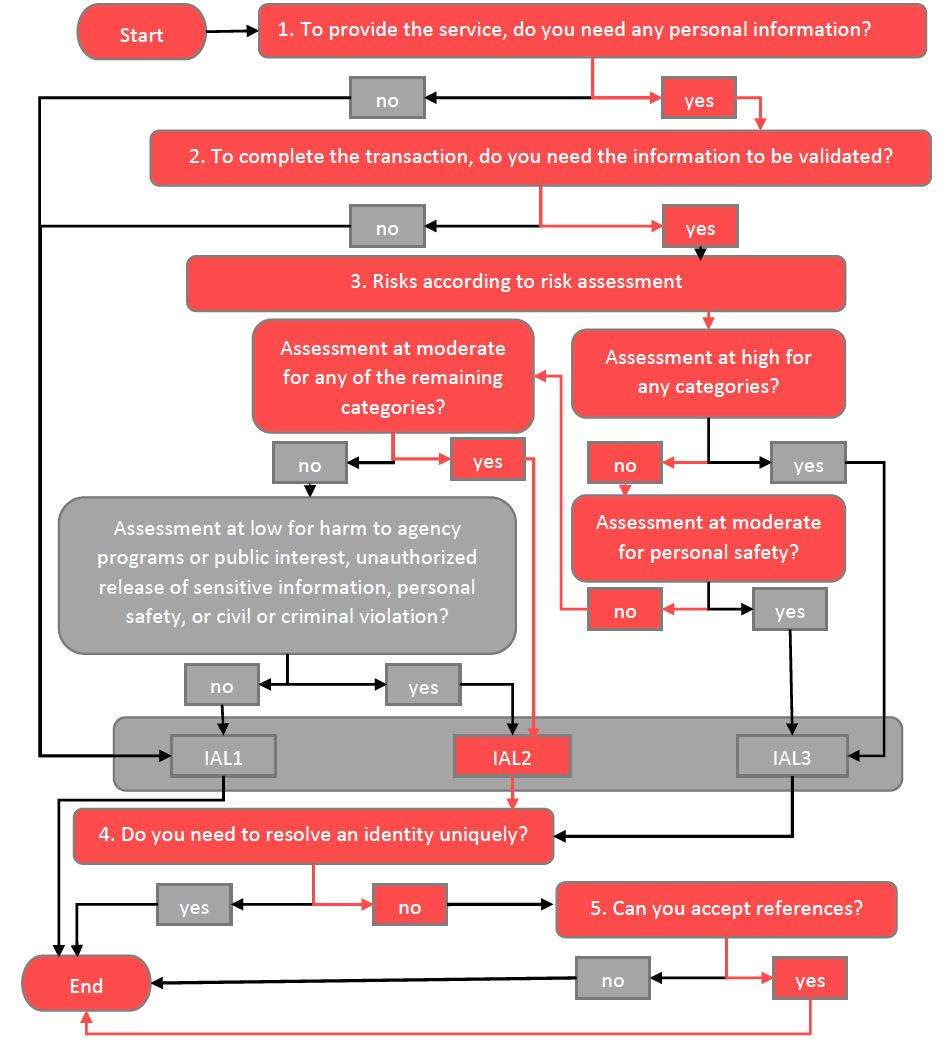
\includegraphics[width=0.9\linewidth]{images/ial_flow_red}
	\caption{Identity Proofing Assurance Flow Chart (\cite{NIST:2017:DIG}, p 27)}
	\label{fig:ialflow}
\end{figure}


In figure~\ref{fig:ialflow} the first question is if PII is needed to provide the service. In our use case, probably sensitive company information is provided therefor yes - personal information is needed. Some of the attributes that are provided have to be validated and can not be self-asserted attributes only therefore the second question can also be answered with - yes.  The next step covers potential impacts of identity proofing. The two threats that is considered here are the most primary identity proofing failures from the view of the user and the company: accepting a falsified identity as true and collecting more information as needed. The before evaluated risks lead to the Identity Assurance Level 2. The two question that are following try to evaluate if a federation is an option. Question four evaluates if the service needs to know the full identity of an user and pseudonymous access even with just a few validated and verified attributes, is not possible. The a answer is no,because in order to reduce the risk of exposure and storing more personal information then necessary a limited set of claims should be accepted. Question five focuses on whether the service should be able to access full attribute values. That does not mean that all attributes have to be delivered in claims, but it should be considered. Since, yes was picked at the question the service is an excellent candidate for a federated infrastructure [cf. (\cite{NIST:2017:DIG}, pp. 28)]. 

\begin{figure}[h]
	\centering
	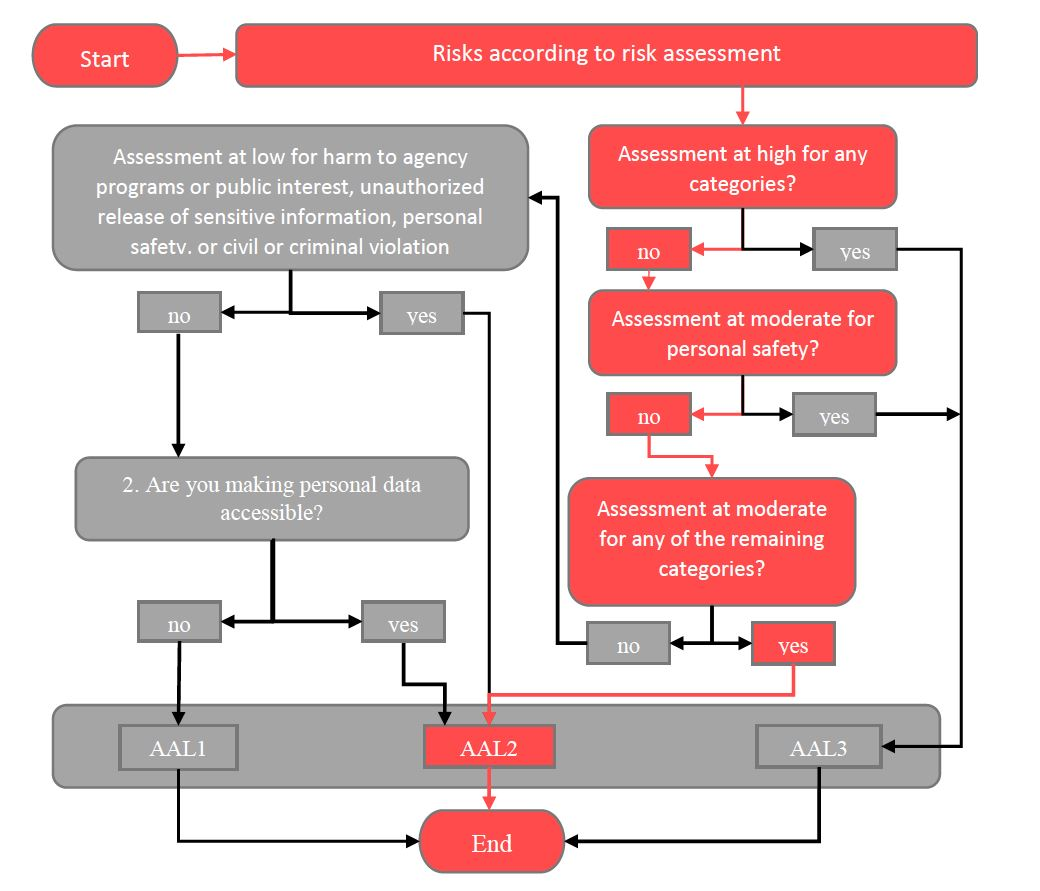
\includegraphics[width=0.9\linewidth]{images/aal_flow_colored}
	\caption{Authentication Assurance Flow Chart (\cite{NIST:2017:DIG}, p 30)}
	\label{fig:aalflow}
\end{figure}

The next flowchart figure~\ref{fig:ialflow} should help to decide on the authenticators necessary for the service. The risks of letting an unauthorized user access information and a compromised account from the risk assessment are taken into account to answer the question. In this use case, sensitive information of the customer are endangered. However, an e-mail filtering report does not have devastating impacts on the customers business, therefore the assessment ends with the AAL2 [cf. (\cite{NIST:2017:DIG}, pp. 30)].  

\pagebreak[4]

\begin{figure}[h]
	\centering
	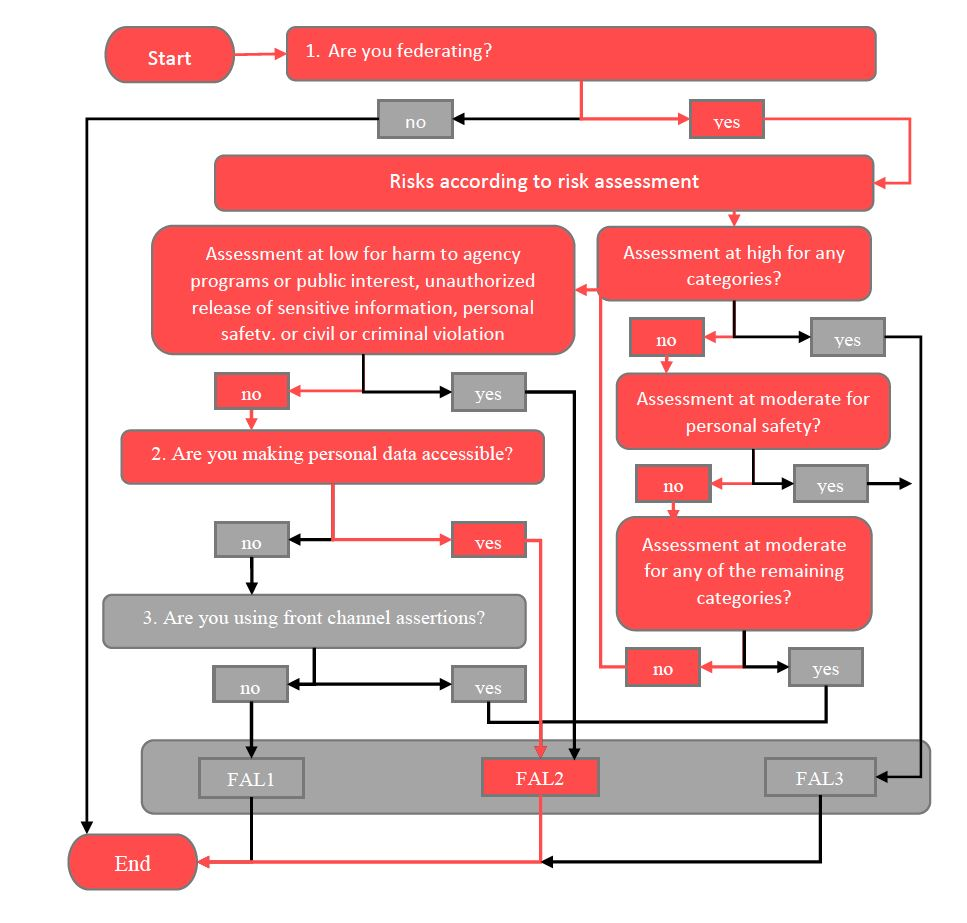
\includegraphics[width=0.9\linewidth]{images/fal_flow_colored}
	\caption{Federation Assurance Flow Chart (\cite{NIST:2017:DIG}, p 32)}
	\label{fig:falflow}
\end{figure}

The last flowchart depicts a federation assurance level flow chart shown in figure~\ref{fig:falflow}. The first question can be answered positivly since a federated service should be considered according to the evaluation in figure~\ref{fig:ialflow}. The next questions are answered according to the conducted risk assessment. This leads to question two, which evaluates if the service will show personal data - yes. The last question leads to Federation Assurance Level 2 [cf. (\cite{NIST:2017:DIG}, pp32)]. 

\pagebreak[4]
\section{Results}
\label{resultSummary}

This initial assertion should give a general direction in which security controls should be in place passed on the different LOA. The risk assessment helps to balance out security and usability, to give the user the best experience possible when using the application. The Risk assessment done in this chapter is based on 'Guide for Conducting Security Risk assessment' by NIST (2012) and on an example done by Hudson (2015). The result indicates which LOA is best suited for the use case presented. The conducted assessment was an initial assessment to create a risk profile. An semi-quantitative assessment approach was used for the assessment and the analysis approach was threat-oriented. The outcomes of this assessment where then compared table \ref{tab:maxImpacts}. After the initial risk assessment with just a view threats that were analyzed the associated assurance level for identity proofing would be \textbf{two}, for authentication risk, it would be \textbf{two}, and for federated risk, the assurance level would be \textbf{one} [cf. (\cite{NIST:2017:DIG}), (\cite{NIST:2018:RMF}), (\cite{Hudson:2015:SecurityRisk})].

Additionally three different flowcharts from were evaluated based on 'Digital Identity Guidelines' by Grassi, Garcia, \& L. (2017). The identity assurance flow chart shown in figure \ref{tab:ial} suggest level \textbf{two} as the right level and indicates that the use case would be a good candidate for federation. The second flowchart shown in figure \ref{tab:aal} also suggest the same level of assurance for authentication as evaluated before - \textbf{two}. Only the last flowchart differs from the previous result. The suggested assurance level for federation is \textbf{two} [cf. (\cite{NIST:2017:DIG})]. 
 
\chapterend

  %%%%%%%%%%%%%%%%%%%%%%%%%%%%%%%%%%%%%%%%%%%%%%%%%%%%%%%%%%%%%%%%%%%%%%%%%%%%%
\chapter{Implementation of Identity Management}\label{chap:implementation}
%%%%%%%%%%%%%%%%%%%%%%%%%%%%%%%%%%%%%%%%%%%%%%%%%%%%%%%%%%%%%%%%%%%%%%%%%%%%%
\chapterstart

 Based on this risk assessment a small solution representing the identity management is implemented. The procedure of conducting a risk assessment should help developers to choose appropriate authentication and authorization methods for a particular use case. The chapter is split up into two parts. The first part describes how the architecture of the solution was chosen and the second part explains how the identity management of the solution works. 
 
 
 \section{Architecture}
 \label{architecture}
 
 The Sakimura et al. (2014) explains that modern applications have different requirements than their predecessors, due to new distributed architectures that allow enterprises to be more flexible. Cloud or microservice architectures require different interactions between applications.The below (figure~\ref{fig:architecture-identityserver}) shows the most common interactions for modern applications [cf. (\cite{Sakimura:2014:OpenIDConnect})].

 
 For example, a browser might call a Web App, and a Web App calls a Web API or perhaps a Native App calls a Web API, which is calling another Web API. Each application has to implement security functions to maintain a secure flow throughout these interactions. Implementing this security features for each involved application leads to a lot of duplicated code and inconsistencies. A different approach to implement security throughout these flows is using a token service. A token service brings the benefit of being able to encapsulate these security functions. Security functions can be updated and hosted at a single point which prevents duplicated functions across applications and security flaws. The advantages of a token service or token based application are also outlined in the section \ref{tokenBasedAuthentication}. Furthermore, the chapter \ref{tokenBasedAuthentication} hold examples of JSON Tokens and how they are asserted. The concept of JSON Tokens is fundamental in token-based authentication systems and ensures confidentiality and integrity [cf. (\cite{Sakimura:2014:OpenIDConnect})].
 
  \begin{figure}[h]
 	\centering
 	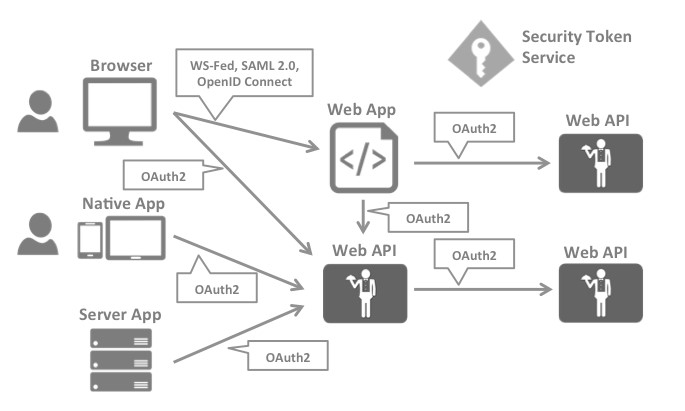
\includegraphics[width=0.9\linewidth]{images/architecture-identityserver}
 	\caption[Architecture IdentityServer4]{Architecture IdentityServer4 (\cite{Brock:2018:ID4}}
 	\caption{Architecture IdentityServer4 (\cite{Brock:2018:ID4})}
 	\label{fig:architecture-identityserver}
 \end{figure}

 Based on the chapter \ref{riskassessment} the architecture of the authentication system for the use case described in chapter \ref{usecase} is chosen. The LOA for identity proofing should be two, according to the risk assessment. Other LOA for identity proofing are covered in chapter \ref{identityProofing}. The second level of assurance for identity proofing suggests that no real-world existence of the claimed identity has to be present. The presentation of the real-existence can be either remote or physical. This means for our example that the user does not have to be physically present, which would be the case for passport controls. The users can sufficiently prove their identity remotely. Additionally to the LOA figure~\ref{fig:ialflow} suggest, in consideration of a unique resolvent of an identity, that accepting references is ok. This means that not always a full presentation of an identity is needed and that for this use case the usage of claims is acceptable. The usage of claims also implies that a federation solution is recommended. 
 
 The federation solution should furthermore offer SSO because of the requirements described in \ref{usecase}. The Single Sign-on solution uses OAuth and OpenID Connect given the facts that were pointed out in \ref{singlesignon}. With help of the risk assesment the kind of tokens which should be provided by the token service are selected. According to the risk assessment, the federation assurance level which is suggested is two. The second federation assurance level states that assertions are required; like the OpenID Connect ID Token. Moreover, the tokens have to be encrypted with a public key of the RP. Therefore the solution will use a token service with bearer tokens.
 
  In order to receive a token from the token server, users have to successfully prove their identity. In order to prove their identity, the users have to provide valid credentials to authenticate at the service. The authentication assurance level analyzed in the chapter \ref{riskassessment} helps to choose the factors for the solution. According to this initial risk assessment, the level of assurance should be two. Other LOA are described in chapter \ref{authentication}. The second level of authentication assurance suggests using at least two distinct authentication factors and the use of strong cryptographic techniques. However, the first level for authentication will be used in this solution, because two distinct authentication factors would typically just be used for really sensitive personal data like in a bank app. The first level of assurance for authentication suggests the use of one authentication factor which should be sufficient for this application.
 
 The risk management and previous observations lead to a simple modern architecture consisting of an Identity Server, an API and an Angular Application. The Identity Server is using bearer tokens and provides Single Sign-on. The API is just accessible with a valid token. If a valid token is provided, it returns protected resources. In this case, the API application also serves as a resource server. Last but not least, the solution includes simple Angular App which provides a login functionality and a page that is just accessible with a valid token.
 

\section{Implementation}

The implementation is based on the architecture described in \ref{architecture}. The languages chosen for the example application are C\# and Angular 2. The solution is created with a very useful ASP.NET framework called Identity Server4. Identity Server4 uses the specifics of OpenID Connect and OAuth 2.0 to enable authentication and authorization related features. Features include authentication as a Service, which provides a centralized login logic for all applications, Single sign-on, Access Control for APIs and Federation Gateway. The Identity Server 4 will be used as a Token Server in the practical part [cf. (\cite{Brock:2018:ID4})]

The project illustrating the use of Identity Server and the benefits of OpenID Connect an OAuth is a Visual Studio Project mostly written in C\# and Typescript. The project example for Identity Server includes four different projects:

\begin{itemize}
	\item Identity Server - The Identity Server is a ASP.NET Core Project with basic implementation of an Identity Server which serves as a Token Server. 
	\item ProjectApiNetCore - This application is a ASP.NET Core 2.0 API Application with basic API that returns the users claims if he is authenticated.
	\item Angular Client - The Angular Client is a ASP.NET Core MVC Angular Project used as a client that can be accessed by an End-User who can authenticate with the Identity Server and requests protected resources of the API ProjectApiNetCore.This project uses the Implicit Code Flow. 
\end{itemize}



\paragraph{Identity Server}

This project is using the IdentityServer4 library by Brock Allen and Dominick Baier. The Project works as a Token Server which means that the Identity Server Project is responsible for the authentication of the user, managing the identities and provide and approve tokens. Furthermore, the Identity Server implements different Authentication Flows.


\begin{figure}[h]
	\centering
	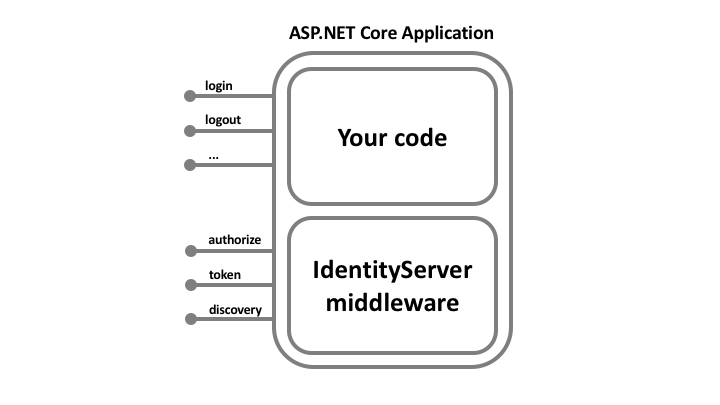
\includegraphics[width=0.6\linewidth]{images/middlewareIdentityServer}
	\caption{IdentityServer Middleware}
	\label{fig:middlewareidentityserver}
\end{figure}
 

IdentityServer4 adds endpoints of OAuth 2.0 and OpenID Connect to an arbitrary ASP.NET Core application as shown in figure~\ref{fig:middlewareidentityserver}. The identity server can be as complex as the developer wants but Brock \& Baier (2018) recommend to keep the attack surface as small as possible by just including authentication related UI only [cf. (\cite{Brock:2018:ID4})]. 


For the basic setup, the Identity Server has to be added to the StartUp class and to ensure a secure communication a certificate is created to sign the request. For the basic setup, Identity Server provides us with DeveloperSigningCredentials which provides a dummy certificate. In this example application, a real certificate is included. 

\begin{figure}[h]
	\centering
	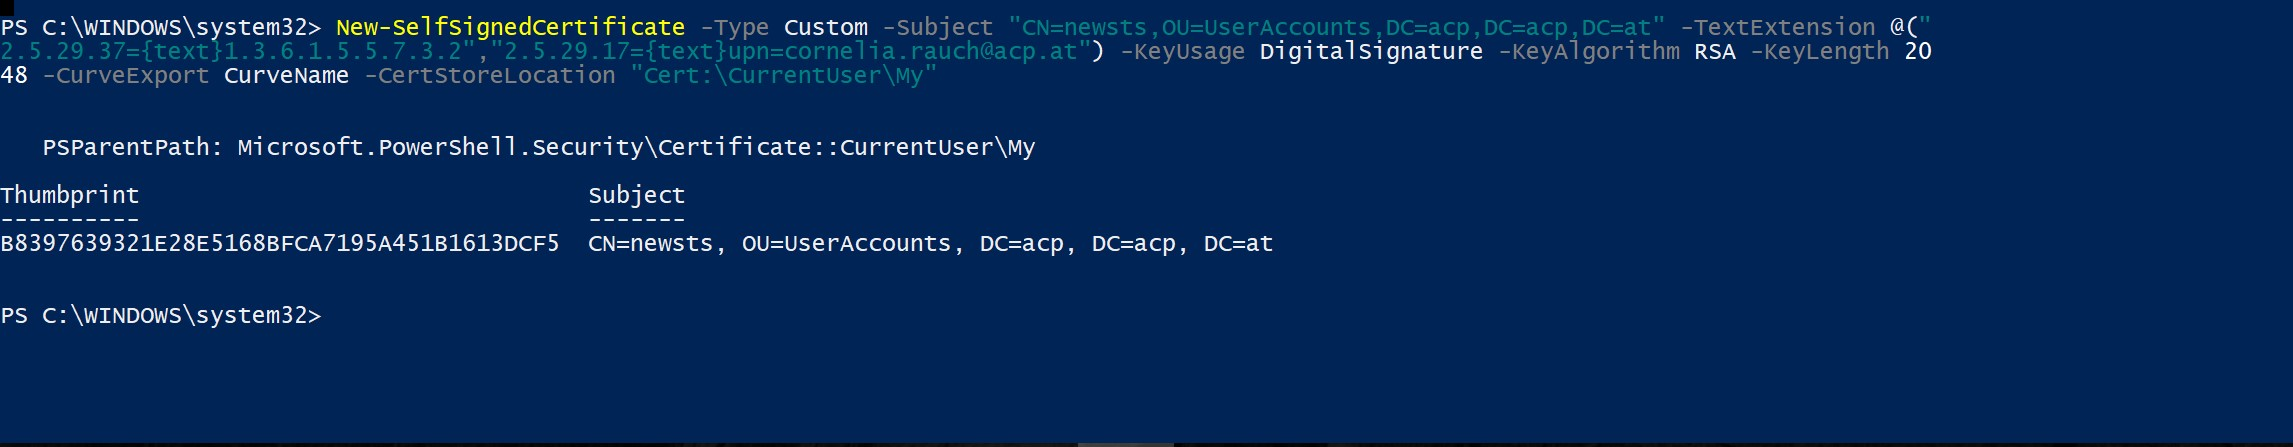
\includegraphics[width=0.9\linewidth]{images/self-signed-certicate}
	\caption{Self signed certificate with Powershell}
	\label{fig:self-signed-certicate}
\end{figure}

The certificate used in this application was created with Powershell as shown in figure~\ref{fig:self-signed-certicate}. The algorithm used in this certificate is RSA. Depending on the algorithm that is used in the certificate a similar hashing algorithm has to be used for the Client Secret.


The API Resources include the available APIs that can be called and included in the scope of a request. The Identity Resources are Resources that can be included in the returning id\_token. The clients are the available clients that can be configured and can use the Identity Server. Those client Configurations indicate which Authorization Flow is used and how to retrieve id\_token, access\_token, and a possible refresh\_token. For simplifying reasons, Identity Server provides an in Memory User Storage which can be used for testing reasons. Other ways to define users are via .NET Core Identity or IdentityServer4 EntityFramework. For the purpose of this implementation this test users where included in the Identity Server application:
\begin{enumerate}
	\item User1:
	\begin{itemize}
		\item  Username: bob
		\item  Password: bob
	\end{itemize} 
	\item User2:
	\begin{itemize}
		\item  Username: alice
		\item  Password: alice
	\end{itemize} 
\end{enumerate}

After the basic setup of the Identity Server, it can be examined if the Identity Server is running correctly by calling the discovery document. The discovery document can be used by the Clients and APIs to retrieve necessary configuration data. The Identity Server has to run at local port 5000 and the navigation path for the browser is:
\url{http://localhost:5000/.well-known/openid-configuration}.

\begin{figure}[h]
	\centering
	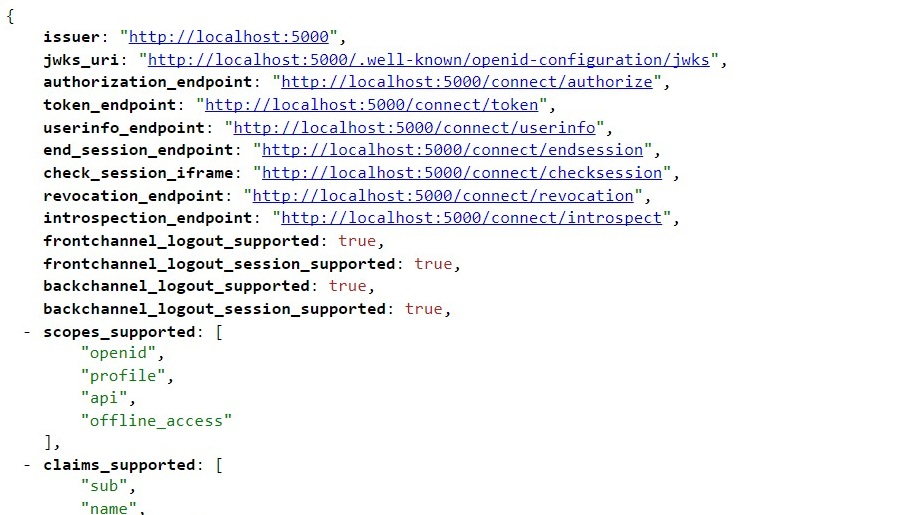
\includegraphics[width=0.8\linewidth]{images/openid-discovery-document}
	\caption{OpenID Discovery Document}
	\label{fig:openid-discovery-document}
\end{figure}
The discovery document shown in figure~\ref{fig:openid-discovery-document} is located at a well-known location and is containing key-value pairs as a JSON structure. The key-value pairs in the discovery document represent multiple endpoints that are used to authenticate a user including URIs of the authorization, token, userinfo and public-keys endpoint. The use of a discovery document brings more flexibility to the protocol. The application should have the discovery URL hard-coded in the application according to (\cite{Google:2018:IdentityPlatform}) the discovery document URL can then be used to fetch endpoints from the document and use them to send an authentication request for example [cf. (\cite{Google:2018:IdentityPlatform})].

The metadata that is seen in \ref{fig:openid-discovery-document} is a mixture of required elements with some recommended ones that are implemented by the Identity Server. The required elements are issuer, authorization\_endpoint, token\_endpoint, jwks\_uri, response\_types\_supported, subject\_types\_supported and id\_token\_signing\_alg\_supported. The issuer, in this case, is this Identity Servers address. The authorization\_endpoint is the URL OAuth 2.0 Authorization Endpoint. The user is redirected to the authorization server's authorization endpoint for authentication and authorization. The authentication request that is sent to the authorization server can have different request parameters. These request parameters are defined by OAuth 2.0 and additional request parameters defined by OpenID Connect. The token\_endpoint is the URL of the OAuth 2.0 Token Endpoint. The RP can request access or optionally refresh tokens from the token endpoint. The user\_endpoint can be used to request additional information concerning the user. The response\_types\_supported is a important information about what kind of response is supported and ultimately what kind of authentication flow can be used based on that information described in chapter \ref{chap:authenticationandauthorization}. The subject\_types\_supported is a list of subject identifier types. Moreover, id\_token\_signing\_alg\_supported is used to find out which JWS is signing algorithm is used to encode the ID token and get the claims of the JWT. The algorithm RS256 must be included [cf. (\cite{Sakimura:OIDCC}, (\cite{Sakimura:OIDCD}))].. 

\begin{figure}[h]
	\centering
	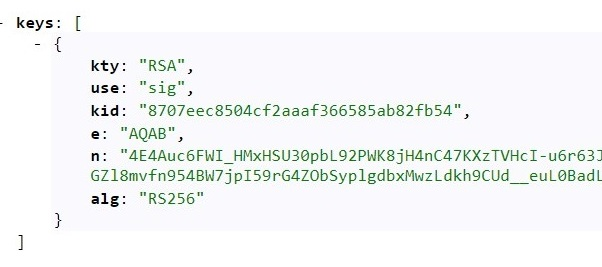
\includegraphics[width=0.7\linewidth]{images/jwkDiscovoryDocument}
	\caption{JWKS Endpint}
	\label{fig:jwkdiscovorydocument}
\end{figure}

The jwks\_endpoint is worth a closer look. JWKS SET is published to the JWKS endpoint. The keys shown in figure~\ref{fig:jwkdiscovorydocument} can be rolled over by periodically adding new keys to the JWK Set. This also indicates if the cryptographic algorithms are configured correctly. For example the message is using the kid of signing key in the JOSE Header to indicate which key has to be used to validate the signature. The algorithm used by the signing party has to be supported by the recipient and can be either an Asymmetric Signature or a Symmetric Signature. 
When using RSA or ECDSA signatures, the alg Header Parameter has to be set to the correct algorithm, and the private key used to sign must be associated with the public key published by the sender. When using MAC-based signatures, the alg Header Parameter has to be set to the correct algorithm, and the MAC key is the octets of the UTF-8 representation of the client\_secret. MAC-based signatures cannot be used by public Clients because they cannot keep secrets.  All metadata types are listed in the specification of OpenID Discovery Document from Sakimura et al. (2014) [cf. (\cite{Sakimura:OIDCD}))]. 

After calling the OpenID discovery document and the JWKS endpoint, one can be ensured that the basic setup of the IdentityServer works. After that a resource that is worth beeing protected by the Identity Server has to be created. 

\paragraph{ProjectApiNetCore}

This ProcjectApiNetcore is an ASP.NET Core application. This application represents the Resource Server and serves the Protected Resources. The example API provides dummy data for the particular request. For easy testing of the API and designing the API, swagger.io is used. Furthermore, swagger.io (\url{https://swagger.io/}) gives a nice developer experience with an interactive API documentation. In addition, it is possible to generate code out of the swagger documentation for different programming languages with tools like NSwag (\url{https://github.com/RSuter/NSwag}).

\begin{figure}[h]
	\centering
	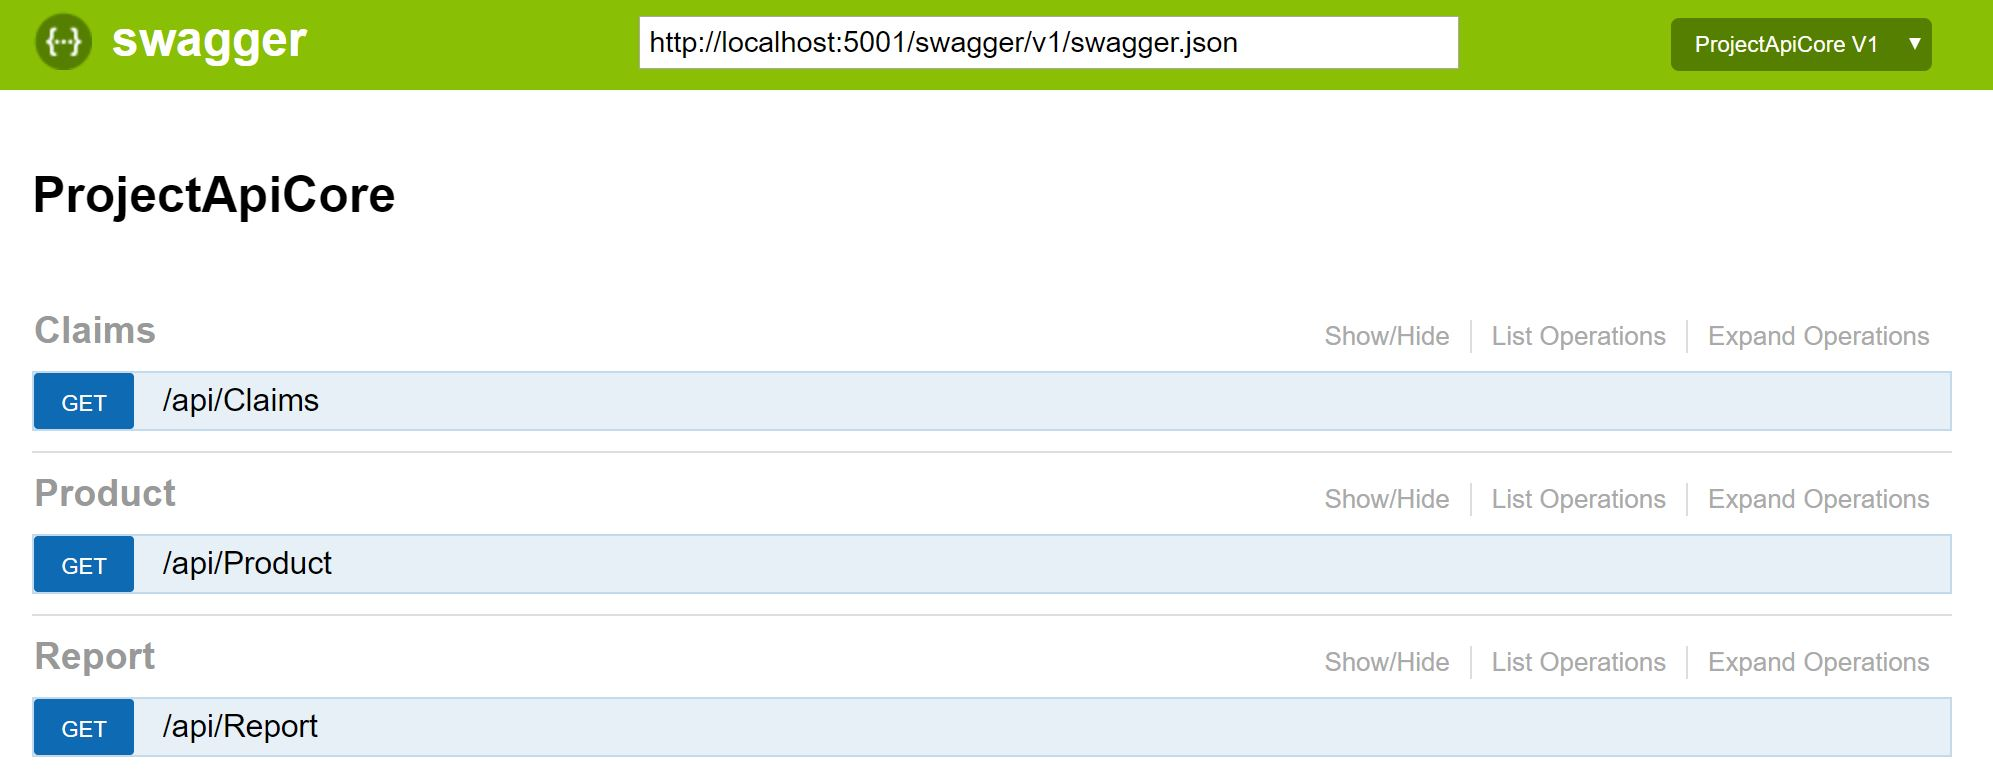
\includegraphics[width=0.7\linewidth]{images/apis}
	\caption{API documentation with Swagger}
	\label{fig:apis}
\end{figure}

All of the routes shown in figure~\ref{fig:apis}, are secured with the help of the IdentityServer4. AccessTokenValidation NuGet package. Each Controller gets an Authorize annotation. 
To configure the right authentication method, ASP.NET Core 2.0 offers the possibility to add the authentication to the pipeline with Dependency Injection via the method Configure Services in the Startup.class.
In the StartUp class of the API Project the AddAuthentication with the Value "JwtBearerDefaults.AuthenticationScheme" makes "Bearer" the default authentication scheme. With the AddIdentityServerAuthentication it is defined which Token server can be used to validate the incoming token and make sure that this token is from a trusted issuer. It adds the Identity Server access token validation handler into DI and also it is checked if the token is valid to be used with this API (aka scope). Adding UseAuthentication to the Configure method int the Startup class adds the authentication middleware to the pipeline so authentication will be performed automatically on every call into the host.  Multiple authentication schemes can be used. A list of authentication schemes is then passed to the Authorize attribute separated with a comma. The default scheme results in the HttpContext.User property is set to that identity. After adding the Authentication logic to the API Project, the resources should be protected now. To check if the resources are protected the Swagger documentation can be used. Therefore navigate to \url{http://localhost:5001/swagger/v1/swagger.json} and try out one of the methods shown in figure~\ref{fig:apis}. This should result in a 401 Unauthorized HTTP response code.


\paragraph{Client}The client represents the UI of the 'Security Assessment Portal' with the initial E-Mail-Filtering functionality. The project is an Angular Solution that follows the Implicit Code Flow described in chapter \ref{OAuthAndOpenID}. The Implicit Code Flow is chosen over the other Code Flows based on the type of application, level of trust and the user experience that should be provided. The first decision is based on rather the machine that hosts the application is also the resource owner. If this is the case no end-user authorization is needed. In this use case the resource owner is accessible over the API we provided which is hosted on a different server. If the application is a regular web app the Authorization Code Flow would be recommended. However since the client hosted is a Angular SPA the Implicit Code Flow should be used. The application directly receives an access token and no additional round trips are needed to exchange an received authorization code. The implicit code flow does not return a refresh token because it can not be kept secret but there is the possibility of a silent authentication. The silent authentication is initiated with a request to the authentication request with the parameter 'promt=none'. On success the client is redirected to the redirect\_uri with an successful authentication response. If the user is not already logged on the client is redirected to the redirect\_uri with an error response [cf. \cite{OAuth:2018:Flow}].  

\begin{figure}[h]
	\centering
	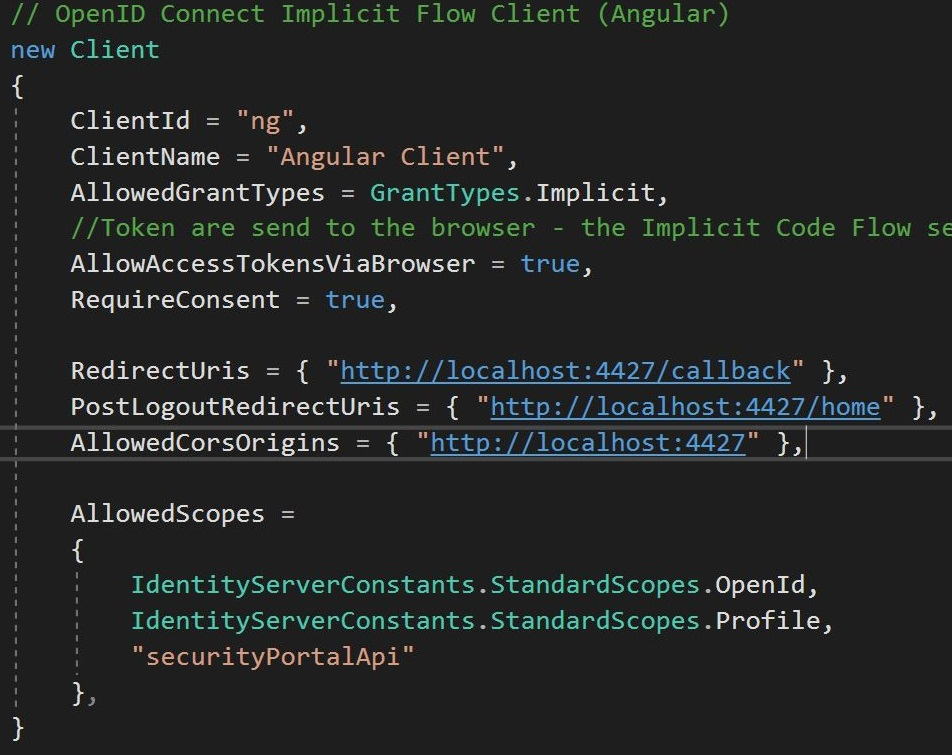
\includegraphics[width=0.8\linewidth]{images/implicit_code_flow}
	\caption{Implicit Code Flow - Identity Server Configuration}
	\label{fig:implicitcodeflow}
\end{figure}

For the Implicit Code Flow, the Identity Server has to define a Client that Allows the Grant Type Implicit as shown in figure~\ref{fig:implicitcodeflow}. The defined Client can be identified with the ClientId. This particular Client also requests the explicit consent of the Client for the requested Scopes. In this case, the Client is allowed to request the well known Scopes OpenId and Profile. In order to receive an id\_token and therefore configure OpenId Connect the scope OpenId has to be requested. The Profile scope gives general information about the user. Also, an API scope is added for ‘securityPortalApi’, which represents the API Project holding the Resources. 




AllowAccessTokensViaBrowser makes sure that the access\_token can be directly returned to the browser after the client authenticates itself. AllowCorsOrignins allows the given resource to make Cross-Origin-Requests to the Identity Server. Cross-Origin-Request is a request that is made from another domain outside the domain from which the first resource was served. Furthermore, the RedirectUris have to be present, in order for the Identity Server to know where to return after the login attempt was successful. 


In the Angular Solution, a service to handle authentication was created. The service handles requests to the API which is hosting the protected resources. The Angular solution uses the ‘oidc-client’ library that is suggested by the Identity Server framework to handle authentication requests. To call the Identity Server the following setting are used, shown in figure~ \ref{fig:implicitcodeflowangular}.

\begin{figure}[h]
	\centering
	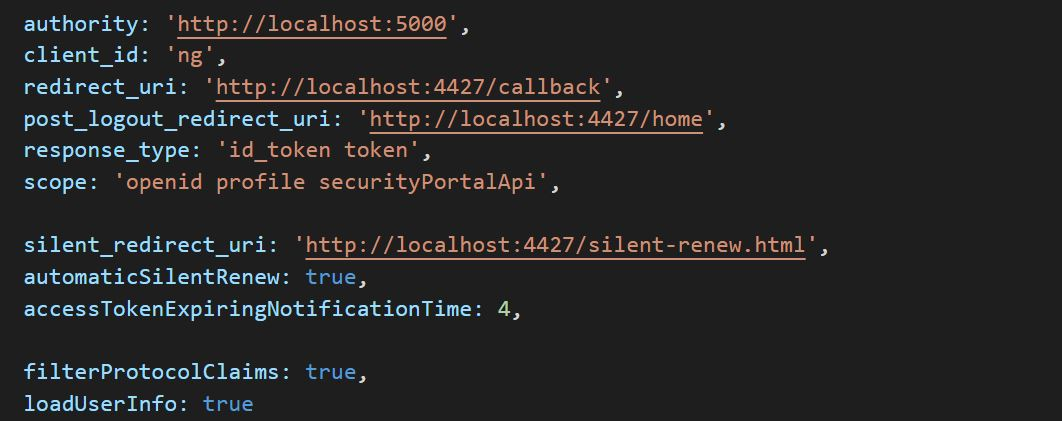
\includegraphics[width=0.8\linewidth]{images/implicit_code_flow_angular}
	\caption{Implicit Code Flow - Angular}
	\label{fig:implicitcodeflowangular}
\end{figure}


The client\_id in the Angular solution has to be the same as the ClientId configured in the Identity Server project. The same is true for the redirect\_uri and post\_logout\_ redirect\_uri. Otherwise, the request would result in an error. For example, if a scope is requested which does not exist accordingly to the Identity Server, an invalid scope exception is thrown. Furthermore, the response\_type has to be according to the used Authorization Flow in the in IdentityServer's client configuration. In the Identity Server Solution, the  Implicit Code Flow was configured, therefore "id\_token token" was defined. The response of these response types will include an access token, an access token type and an id\_token.  

\begin{figure}[h]
	\centering
	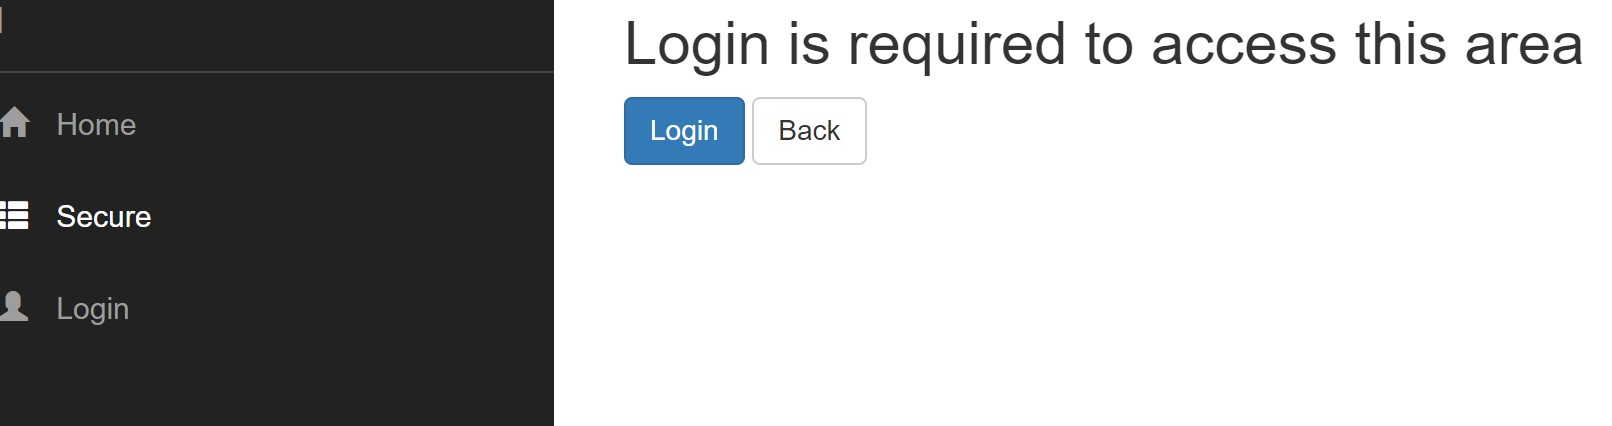
\includegraphics[width=0.8\linewidth]{images/secure_page_requires_login}
	\caption{Secure Page Login}
	\label{fig:securepagerequireslogin}
\end{figure}

For the Client to receive an id\_token and in this example an access\_token from the Authorization Server (Identity Server Project), the client has to prepare an Authentication Request and send it to the Authorization Server. The Angular Client has two possible ways to trigger the login with the Identity Server. In the navigation on the left-hand side there is a Home Page that can be accessed by everyone, then there is a Secure Page that just can be accessed by logged in users and the Login Page, which automatically triggers a request to the Authorization Server.



The figure~\ref{fig:securepagerequireslogin}, shows the Menu of the application. If the user tries to access the Secure Page without being logged in he is redirected to the "Login is required" Page. In order to access the secure area, the End-User has to authenticate with the Authorization Server.
To authenticate with the Authorization Server the user has to press the Login button. After the Login button is pressed, the End-User is redirected to the Authorization Server Login Page. The design of this screen can be adjusted in the Identity Server Project. 

\begin{figure}[h]
	\centering
	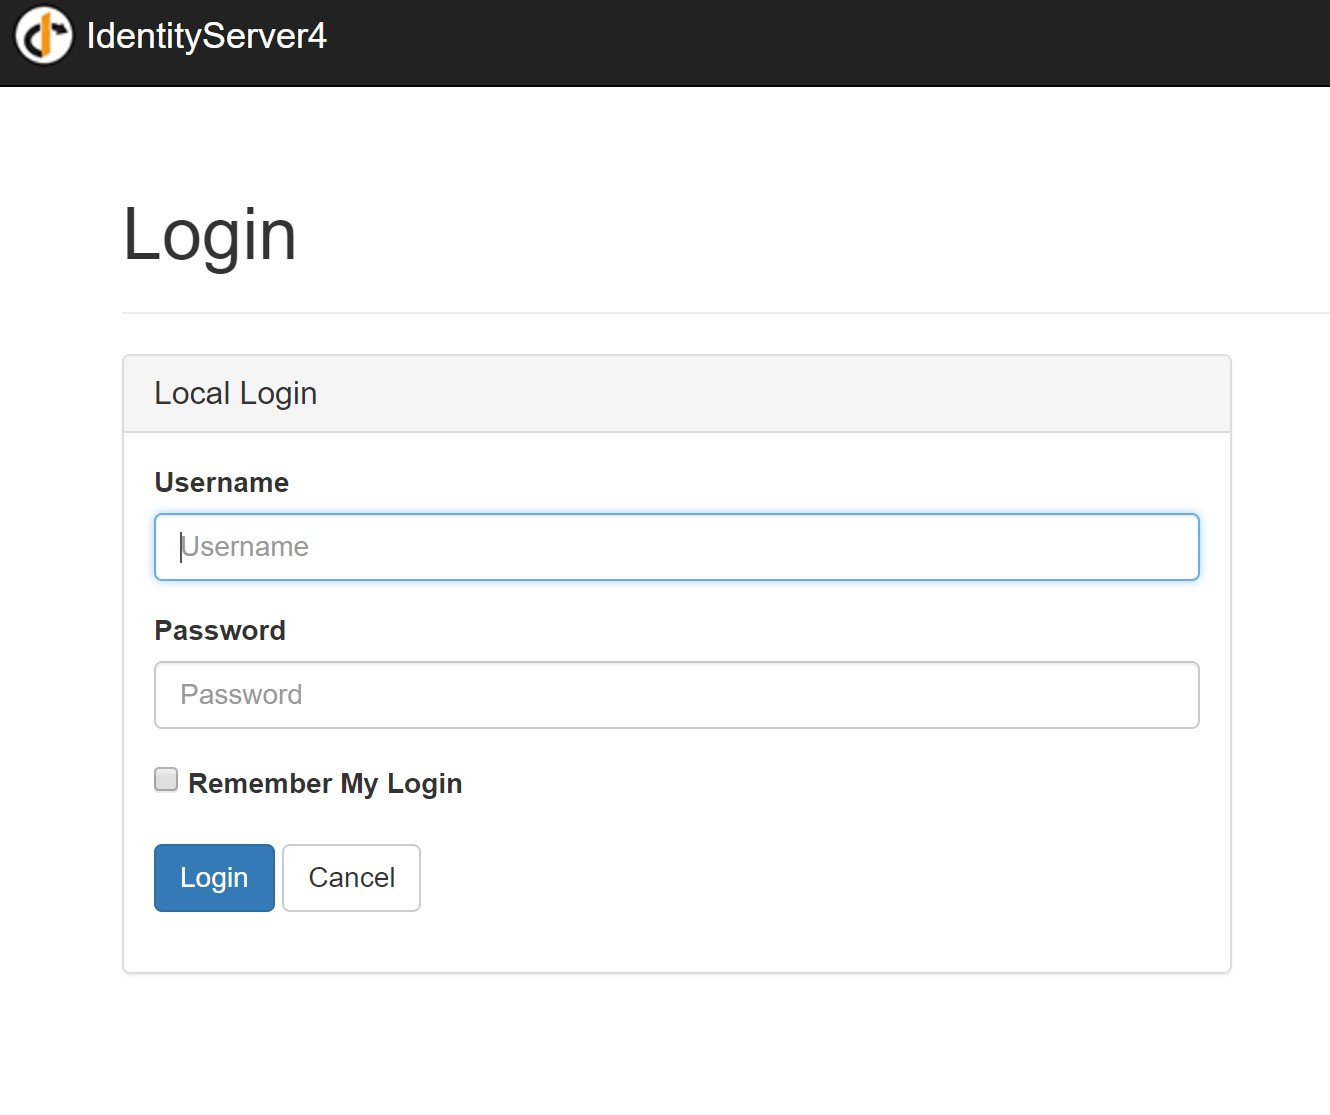
\includegraphics[width=0.7\linewidth]{images/login_identity_server}
	\caption{Login Mask Identity Server}
	\label{fig:loginidentityserver}
\end{figure}


The (figure~\ref{fig:loginidentityserver}), shows the form where the end-user can log in with the end-user’s credentials. In the Identity Server Project, two test-user are registered. Therefore either Alice or Bob can currently log in to the application and view the secured Page. 
The Authorization Server can also request consent from the User for the requested Claims. In the Identity Server Project, it is configured that the consent of the End-User is required. In consequence of this configuration, the user is prompted an additional screen. This screen is shown in figure~ \ref{fig:consentscreen}, it would not appear if the consent was not required by the identity server. 

\begin{figure}[h]
	\centering
	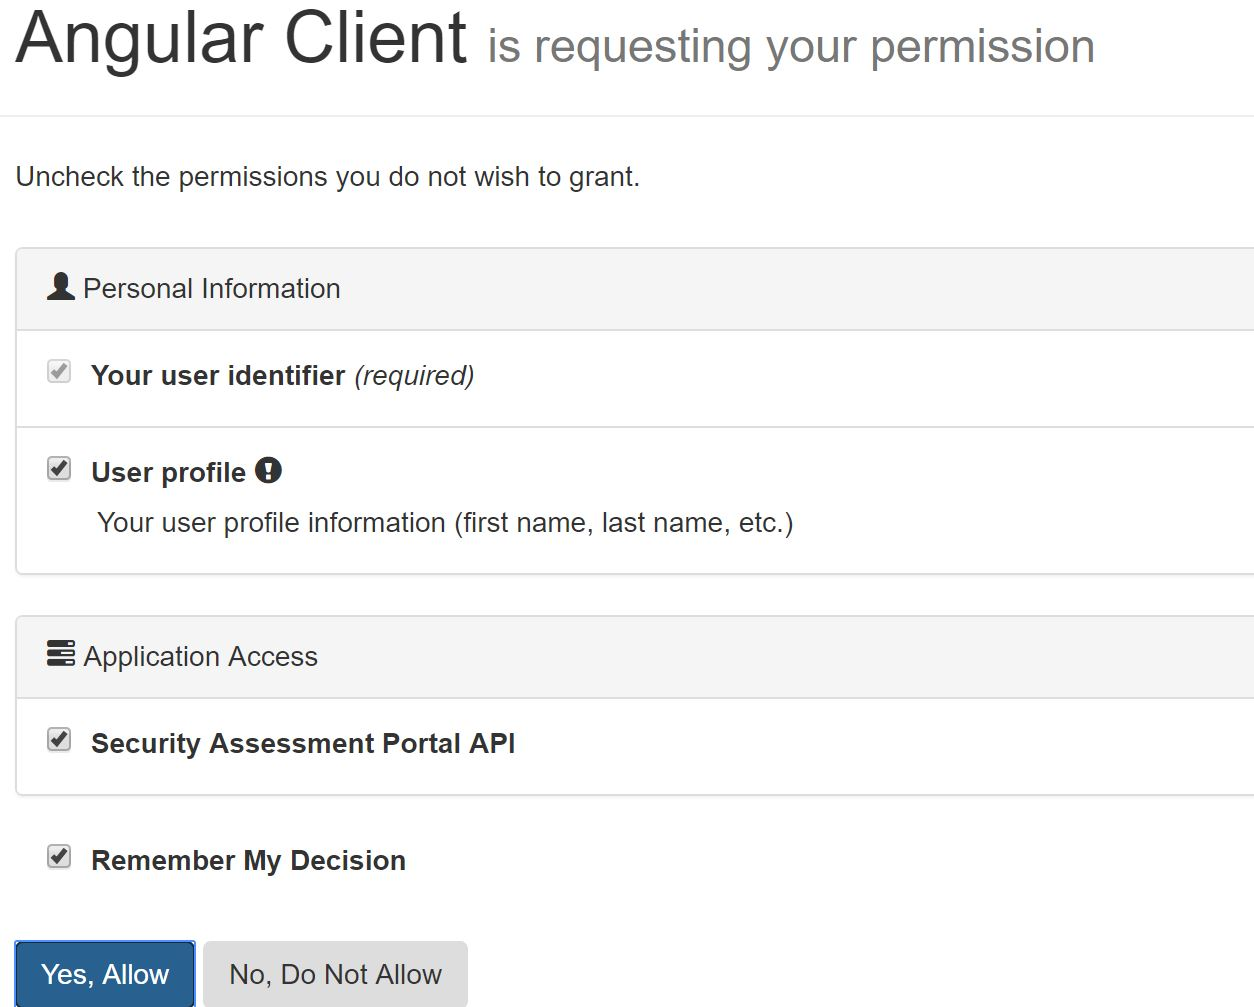
\includegraphics[width=0.7\linewidth]{images/consent_screen}
	\caption{Consent Screen}
	\label{fig:consentscreen}
\end{figure}


The Angular Application is requesting consent for the requested scopes openId, profile and securityPortalApi. The openId Scope is required because otherwise, we would not be able to receive an id\_token. User Profile gives additional information about the User, and the  Security Assessment Portal API is a custom API that was added to the scope and allows the user to make requests to this API and the protected resources. 


After the End-User has given its consent, the End-User gets redirected back to the Client with an id\_token and an access\_token. The id\_token can be validated and an End-User’s Subject Identifier is retrieved.

If the authentication with the Authorization Server was successful the end-user is now authenticated. As an authenticated user the end-user can now also access the Secure Page. With access\_token the received access token calls to the custom API Project can be executed. For example, the claims of the user that are correlating to the scopes can be received and put in a useful context as seen in figure~\ref{fig:claims}.


\begin{figure}[h]
	\centering
	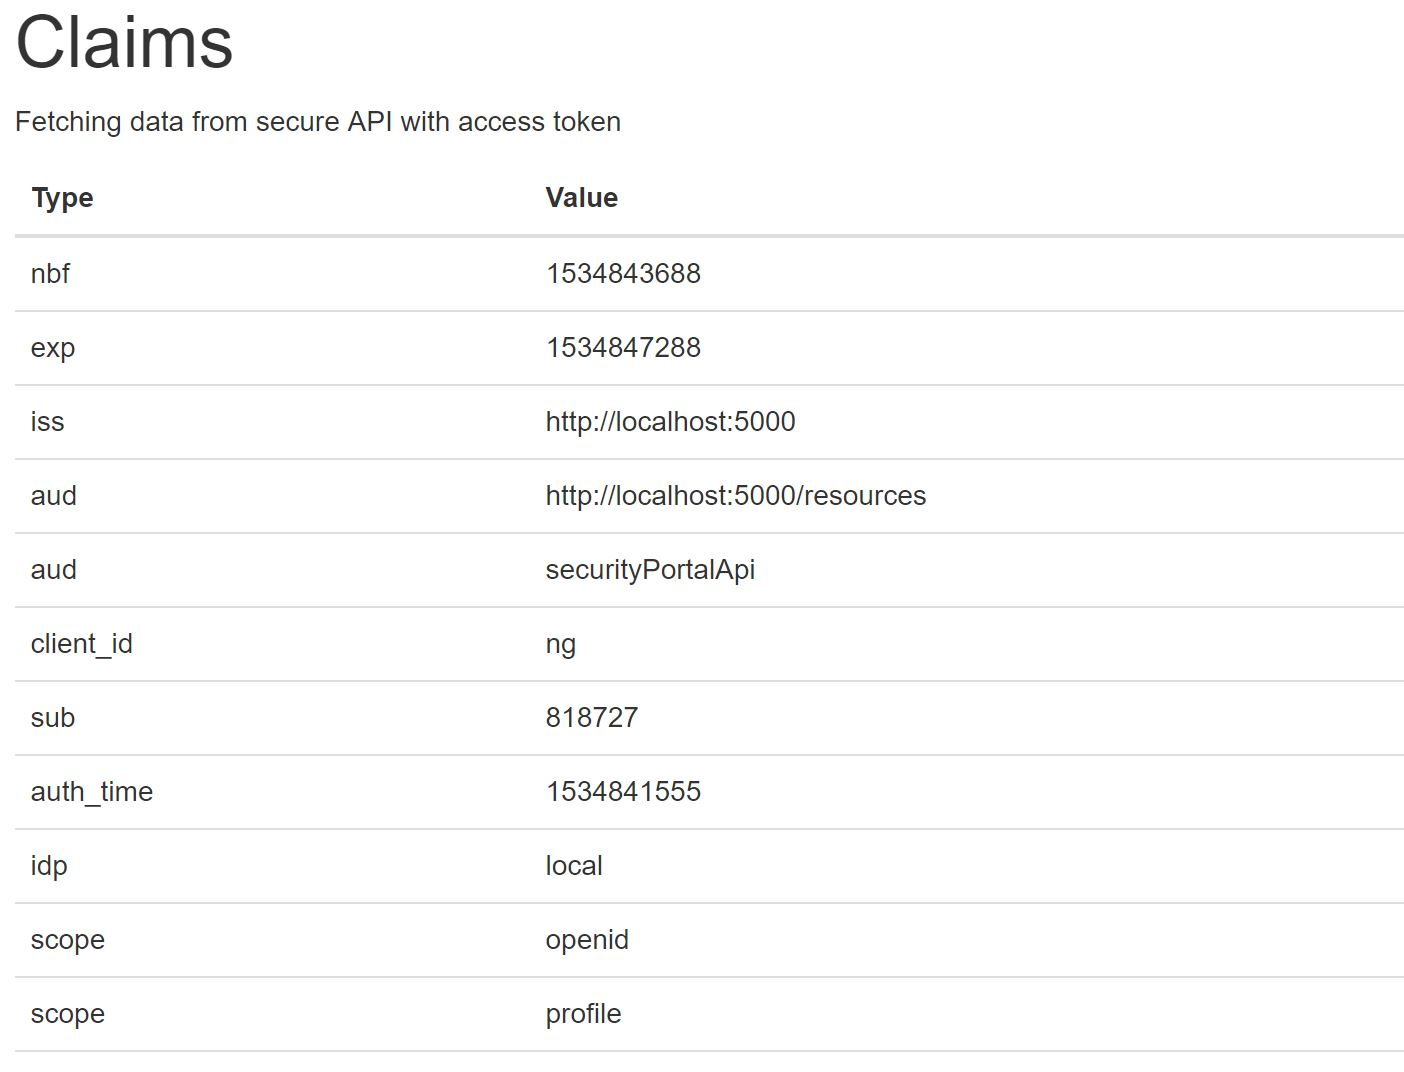
\includegraphics[width=0.7\linewidth]{images/claims}
	\caption{Claims}
	\label{fig:claims}
\end{figure}
 
 \pagebreak[4]

This complete example could be a possible implementation of the authentication for the described use case in section \ref{usecase}. Now it would also be possible for an external user (customers) to access the application without a domain account. If customers also choose to use other products of the companies, no new account is required because the same identity server can be used. The personal data of the customers stays in the company and is not given to any third party. With the use of token-based authentication, it is easy to manage the session of end-users, and the user can stay logged in the application (single-sign-on). The use of bearer tokens gives appropriate security and the implicit flow used to deliver the token makes it very light-weighted for single page application. The separated API is also convenient because it might be used for multiple purposes.

\chapterend

  %%%%%%%%%%%%%%%%%%%%%%%%%%%%%%%%%%%%%%%%%%%%%%%%%%%%%%%%%%%%%%%%%%%%%%%%%%%%%
\chapter{Conclusion and Outlook}\label{chap:conclusion}
%%%%%%%%%%%%%%%%%%%%%%%%%%%%%%%%%%%%%%%%%%%%%%%%%%%%%%%%%%%%%%%%%%%%%%%%%%%%%
\chapterstart

Taking on a new project takes a lot of consideration and planning. The planning includes thoughtful consideration of the security and privacy measures which should be established to create trustworthiness. An essential part of trustworthiness is identity management. Identity management includes ensuring confidentiality, integrity, and availability. 

Chapter two of this thesis focuses on a careful examination of identity management, especially under three different angels identity proofing, authentication, and assertion. Moreover, the difference between using token-based and server-based authentication is analyzed. In token-based authentication systems, it is by far more comfortable to handle sessions, while in server-based authentication systems, this can be challenging tasks. Particular for a single-page application which typically uses an Application Programming Interface hosted on a different server session management can lead to overhead in server-based authentication systems. The thesis also explains the benefits of using a federation system for Single Sign-on and introduces two possible federation systems for Single Sign-on. The two systems which are explained are SAML and OpenID Connect. Both of the systems provide the service of Single sign-on, but ultimately OpenID Connect provides a lighter weighted approach for mobile and single page applications.

The third chapter undertakes the task of finding the best available authentication and authorization methods for a defined use case that requires a Single Page Application and a separated Application Programming Interface. A mature part of reaching this goal was the risk assessment of a use case which was described beforehand. The risk assessment examines different technical threats and rates and determines the risk of each threat according to an existing approach described in the 'Guide for Conducting Risk Assessment' by NIST (2012). Furthermore, flowcharts were consulted which should help with the decision of choosing an appropriate Level of Assurance and if federating the solution should be considered. This risk assessment leads to three different assurance level which can be categorized into identity proofing, authentication, and assertion. 

Based on the level of assurance determined by the conducted risk assessment a solution was created which is an example of the identity management system developed for an use case. The solution is described in chapter four and was based on the knowledge gained from the related work part and considered the outcome of the risk assessment. This leads to a solution with a stand-alone identity server providing a token service, a separate Application Programming Interface which can host private information and a Single Page Application. 

In my opinion, the risk assessment was helpful but should be conducted to a greater extent for a real-life application. Furthermore, the risk determination was difficult because the values of the assessment approach were described very vague in the 'Guide for Conducting Risk Assessment' by NIST (2012), there was no point of reference for assigning the right values. Nevertheless, the risk assessment gave some excellent pointers and made decisions more manageable. For example, it was easier to decide rather to use bearer assertions or holder-of-key assertions. The implementation of the identity management system which was based on the risk assessment is a very feasible way to implement a token service from scratch including the security controls from the risk assessment. The IdentityServer4 framework was very helpful for building the token service, but I would not recommend using the framework without extended knowledge of the OAuth 2.0 and OpenID Connect specification. For example, to implementation and validation of JWT's for an OpenID Connect identity management application, one should know which algorithms are appropriate to use. Additionally, if the solution in chapter four would be further developed, another risk assessment should be conducted. The key to successful risk management is documentation, review and improvement.

\chapterend


  \appendix
  %%%%%%%%%%%%%%%%%%%%%%%%%%%%%%%%%%%%%%%%%%%%%%%%%%%%%%%%%%%%%%%%%%%%%%%%%%%%%
\chapter*{Acronyms}
\label{chap:acronyms}
%%%%%%%%%%%%%%%%%%%%%%%%%%%%%%%%%%%%%%%%%%%%%%%%%%%%%%%%%%%%%%%%%%%%%%%%%%%%%
% Which one will be the longest ...?
% ABCDE --> \begin{acronym}[ABCDE]
\footnotesize
\begin{acronym}[ABCDE]
 \acro{AEAD}	{Authenticated Encryption and Associated Data}
 \acro{API}{Application Programming Interface}
 \acro{ASP}{Authentication Service Provider}
 \acro{CEK}{Content Encryption Key}     
 \acro{CSP}{Credential Service Provider}
 \acro{DI}{Dipendency Injection}
 \acro{GPS}{Global Positioning System}
 \acro{HMAC}{Keyed-Hash Message Authentication Code}
 \acro{HTTP}{Hypertext Transfere Protocol}
 \acro{HTTPS}{Hypertext Transfere Protocol Secure}
 \acro{IdP}{Identity Provider}
 \acro{IP}{Internet Protocol}
 \acro{IT}{Information Technology}
 \acro{JOSE}{Javascipt Object Signing and Encryption}
 \acro{JSON}{JavaScript Object Notation}
 \acro{JWE}{JSON Web Encryption}
 \acro{JWK}{JSON Web Key}
 \acro{JWKS}{JSON Web Key Set}
 \acro{JWS}{JSON Web Signature}
 \acro{JWT}{JSON Web Token}
 \acro{LDAP}{Lightweight Directory Access Protocol}
 \acro{LOA}{Level of Assurance}
 \acro{MAC}{Media Access Control}
 \acro{MFA}{Multi-factor Authentication}
 \acro{MVC}{Multi View Controller}
 \acro{OTP}{One-time Password}
 \acro{PII}{Personally Identifiable Information}
 \acro{PIN}{Personal Identification Number}
 \acro{PKCS}{Public-Key Cryptography Standard}
 \acro{REST}{Representational State Transfere}
 \acro{RMF}{Risk Management Framework}
 \acro{RP}{Relying Party}
 \acro{SAML}{Security Assertion Markup Language}
 \acro{SFA}{Single-factor Authentication}
 \acro{SHA}{Secure Hash Algorithm}
 \acro{SOAP}{Simple Object Access Protocol}
 \acro{SP}{Service Provider}
 \acro{SSO}{Single-sign On}
 \acro{STS}{Security Token Service}
 \acro{UI}{User Interface}
 \acro{URL}{Uniform Resource Locator}
 \acro{UTF-8}{8-bit USC Transformation Format}
 \acro{WS}{Webservice}
 \acro{XML}{Extensible Markup Language}
\end{acronym}
\normalsize


	\printbibliography[type=book,title={Refernce - Books}]
	\printbibliography[type=article,title={Refernce - Articles}]
	\printbibliography[type=online,title={Refernce  - Online Sources}]
	\printbibliography[type=manual,title={Refernce - Manuals}]
	\printbibliography[type=reports,title={Refernce - Reports}]
	\printbibliography[type=misc,title={Refernce - Misc}]

% Add bibliography to table of contents as "References", at chapter level
% Keep this _after_ bibliography, only then the link in the TOC is correct!
\addcontentsline{toc}{chapter}{References}

\end{document}


%**********************************************************************
%**********************************************************************
